%% 
%% Copyright 2019-2024 Elsevier Ltd
%% 
%% Version 2.4
%% 
%% This file is part of the 'CAS Bundle'.
%% --------------------------------------
%% 
%% It may be distributed under the conditions of the LaTeX Project Public
%% License, either version 1.2 of this license or (at your option) any
%% later version.  The latest version of this license is in
%%    http://www.latex-project.org/lppl.txt
%% and version 1.2 or later is part of all distributions of LaTeX
%% version 1999/12/01 or later.
%% 
%% The list of all files belonging to the 'CAS Bundle' is
%% given in the file `manifest.txt'.
%% 
%% Template article for cas-dc documentclass for 
%% double column output.

%\documentclass[a4paper,fleqn,longmktitle]{cas-dc}
\documentclass[a4paper,fleqn]{cas-dc}

%\usepackage[authoryear,longnamesfirst]{natbib}
%\usepackage[authoryear]{natbib}
\usepackage[numbers]{natbib}
\usepackage{amsthm}
\newtheorem{proposition}{Proposition}

%%%Author definitions
\def\tsc#1{\csdef{#1}{\textsc{\lowercase{#1}}\xspace}}
\tsc{WGM}
\tsc{QE}
\tsc{EP}
\tsc{PMS}
\tsc{BEC}
\tsc{DE}
%%%

\begin{document}
\let\WriteBookmarks\relax
\def\floatpagepagefraction{1}
\def\textpagefraction{.001}
\shorttitle{Prior-Guided Policy Learning for Dual-Arm Alignment}
\shortauthors{S.K. Prakash et~al.}

\title [mode = title]{Prior-Guided Policy Learning for Cooperative Dual-Arm Pre-Assembly Alignment}                      
% \tnotemark[1,2]

% \tnotetext[1]{This document is the results of the research
%    project funded by the National Science Foundation.}

% \tnotetext[2]{The second title footnote which is a longer text matter
%    to fill through the whole text width and overflow into
%    another line in the footnotes area of the first page.}


\author[1]{Surya Prakash S.K}[type=,
                        auid=000,bioid=1,
                        prefix=,
                        role=,
                        orcid=0009-0006-3327-8019]
\ead{d21077@students.iitmandi.ac.in}
% \ead[url]{[www.jkkrishnan.in}](https://www.jkkrishnan.in})
\credit{Conceptualization, Methodology, Software, Validation, Formal analysis, Investigation, Writing -- original draft, Visualization}
%\address[1]{, Street 129, 1043 NX Amsterdam, The Netherlands}
\affiliation[1]{organization={School of Mechanical and Materials Engineering, Indian Institute of Technology},
                addressline={Kamand}, 
                city={Mandi},
%               citysep={}, % Uncomment if no comma needed between city and postcode
                postcode={175005}, 
                state={Himachal Pradesh},
                country={India}}
\author[2]{Sai Teja M}
\ead{majjisaiteja12@gmail.com}
\credit{Conceptualization, Methodology, Software, Validation, Writing -- original draft, Visualization}
\author[2]{Praful Hambarde}[%
   prefix= Dr ,
   suffix=,
   orcid= 0000-0002-7976-9095
   ]
\cormark[1]
\ead{praful@iitmandi.ac.in}
% \ead[URL]{https://www.university.org}
\credit{Methodology, Writing -- review \& editing, Supervision}
\affiliation[2]{organization={Centre for Artificial Intelligence and Robotics, Indian Institute of Technology},
                addressline={Kamand}, 
                postcode={175005}, 
                postcodesep={}, 
                city={Mandi},
                country={India}}
\author[2]{Amit Shukla}[
prefix = Dr,
role = ,
orcid=0000-0002-0537-5851
]
\cormark[2]
\ead{amitshukla@iitmandi.ac.in}
% \ead[URL]{[www.campus.in}](https://www.campus.in})
\credit{Conceptualization, Resources, Writing -- review \& editing, Supervision}
% \affiliation[3]{organization={University of Intelligent Studies},
%                 addressline={Street 15}, 
%                 city={Jabaldesh},
%                 postcode={825001}, 
%                 state={Orissa}, 
%                 country={India}}
\cortext[cor1]{Corresponding author}
\cortext[cor2]{Principal corresponding author}

% \nonumnote{This note has no numbers. In this work we demonstrate $a_b$
%   the formation Y\_1 of a new type of polariton on the interface
%   between a cuprous oxide slab and a polystyrene micro-sphere placed
%   on the slab.
%   }

\begin{abstract}
Cooperative dual-arm pre-assembly alignment requires two manipulators to acquire independent targets and then converge on a shared co-axial configuration. Learning low-level actuation and inter-arm coordination simultaneously from scratch is sample-inefficient, while fixed coordination priors cannot adapt across task phases. This paper presents Gated Prior Composition (GPC), a hierarchical framework trained in two stages: a single-arm reaching policy is first trained under PPO to produce a joint velocity-level differential inverse kinematics mapping and is then frozen, and a coordination policy is subsequently trained against it by Multi-Agent PPO (MAPPO) under Centralized Training with Decentralized Execution. Each agent acts on a 47-D local observation, while per-agent critics condition on a shared 92-D global state. The two policy outputs are combined at every control step through a per-arm gating scalar that the coordination policy accumulates incrementally, so that reliance on the prior is regulated by task phase rather than fixed in advance. The framework is completed by a phase-conditioned reward employing a coupled min-operator over position and orientation error, and by a deployment-time way-point state machine that replaces the training-time snap mechanism. Across 4,096 parallel simulation environments the framework attains 95.9\% reach and 93.9\% alignment success, averaged over three training seeds. Direct sim-to-real transfer to two Kinova Gen3 Lite manipulators yields 93.3\% reach and 90.0\% alignment over 30 hardware trials, with 200~Hz policy inference on a CPU-only platform against a 20~Hz hardware control loop. Results are reported for square and cylindrical peg-in-hole configurations under known object pose.
\end{abstract}

% Graphical abstract omitted (optional for Array).
%\begin{graphicalabstract}
%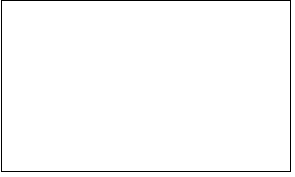
\includegraphics{figs/cas-grabs.pdf}
%\end{graphicalabstract}

\begin{highlights}
\item Frozen reaching prior and coordination policy co-adapt via a learned gating scalar
\item Direct sim-to-real transfer: 93.3\% reach, 90.0\% alignment over 30 trials
\item A fixed 0.9 prior weight gives top training reward but near-zero task success
\item 200 Hz policy inference on a CPU-only platform, 10x the 20 Hz control loop
\end{highlights}

\begin{keywords}
Robot Learning \sep Dual-Arm Manipulation \sep Residual Policy Learning \sep Sim-to-Real Transfer
\end{keywords}


\maketitle

\section{Introduction}
\label{intro}
Robot manipulation plays a key role in industrial automation tasks such as pick-and-place, sorting, and assembly line inspection that are increasingly handled by robotic systems \cite{intro-2}. To accomplish these tasks, robot movements are based primarily on conventional methods such as kinematic and dynamic control, and learning-based approaches, including imitation learning (IL) and reinforcement learning (RL) \cite{intro-3}. Conventional robotic control methods typically involve modular pipelines consisting of sequential planning and control stages. These methods depend on accurate kinematic or dynamic models, which are often complex and difficult to obtain in practice \cite{trajec_conv}. Furthermore, predefined control sequences struggle to generalize across task variations without explicit re-engineering of each module \cite{intro-1}. Advancements in data-driven control techniques such as Learning from Demonstration (LfD) and data collection via teach pendants or tele-operation do not require explicit knowledge of robot dynamics or environmental models to execute tasks. Although these approaches eliminate the dependency on accurate dynamic models, they require a large volume of high-quality data. Consequently, the performance of such systems remains constrained by the availability and diversity of the collected datasets, often making them difficult to scale in complex industrial environments \cite{intro-6}.

To overcome these limitations of data scarcity and human dependence on data collection, reinforcement learning has been introduced as a powerful alternative \cite{intro-8, liu2026review}. Unlike data dependent IL and LfD, RL enables a robot to figure out optimal control policies (state dependent actions) through interaction and exploration with the surroundings \cite{intro-7}. Although RL methods require extensive training time to converge, their capacity to learn optimal control robustly is often more reliable than static data-driven approaches \cite{intro-10}. By optimizing a well-defined reward function, RL-based agents can potentially surpass the performance of human experts and develop resilient recovery behaviors that are not represented in static datasets \cite{intro-9}.

Single arm manipulations based on RL have demonstrated promising results in trajectory optimization \cite{intro-12, intro-13}, path planning \cite{hemalatha2026cleannav}, intelligent pick-and-place \cite{dahmani2025reinforcement, intro-14, intro-15}, obstacle avoidance \cite{intro-16, intro-17}, and human-robot interaction \cite{intro-18, intro-19}. However, complex tasks such as alignment and assembly of components require collaborative manipulation rather than isolated single arm execution. Extending RL from single-agent to multi-agent systems poses significant challenges. In a single-agent environment, an agent is concerned only with the outcomes of its own actions within a stationarity distribution \cite{intro-21}. However, in multi-agent domains, an agent must account for both the consequences of its own actions and the evolving behaviors of other agents. This interaction introduces non-stationarity into the learning process, as the optimal policy of one agent becomes dependent on the fluctuating strategies of its counterparts \cite{intro-20}.

Multi-Agent Reinforcement Learning (MARL) was introduced to address these challenges by explicitly modeling the interactions between multiple decision-making entities \cite{intro-22}. MARL methods are broadly classified along three primary axes. First, by cooperation structure: agents may be fully cooperative, sharing a joint reward to achieve a common goal; fully competitive, operating in zero-sum settings; or mixed, pursuing partially conflicting objectives. Second, by the training and execution paradigm. Independent Learning (IL) treats other agents as part of a non-stationary environment \cite{IPPO}. Centralized Training with Decentralized Execution (CTDE) enables agents to condition value estimation on shared, globally-informed state during training while maintaining independent policies during execution. Centralized Learning (CL) subordinates all agents to a single controlling entity. Third, by communication protocol: communicative agents explicitly share state or intent information, while non-communicative agents must implicitly infer the behaviors of others through observed actions \cite{intro-23, intro-25}. We frame dual-arm coordination as a hierarchical control problem: a frozen single-arm reaching prior is composed with a learned coordination policy responsible for inter-arm alignment. CTDE-style multi-agent training supplies the mechanism for learning this coordination policy, MAPPO's shared global-state critic during training captures inter-arm spatial relationships that a purely per-arm training signal cannot, while per-arm policies remain independently executable at deployment. This decentralized-execution property is retained as an architectural feature, useful for future distributed or independently-controlled arms, rather than a requirement of the present system: both arms are driven from a single CPU-only platform in the hardware experiments reported here (Sec.~\ref{sim_2_real}). While recent heterogeneous-agent CTDE methods like HAPPO \cite{happo/htrpo} offer monotonic improvement guarantees for asymmetric tasks via sequential policy updates, our agents are structurally symmetric, each arm shares identical architecture and observation dimensionality, so MAPPO's simultaneous update is the better-suited choice of the two.

Despite the theoretical advantages of CTDE frameworks like MAPPO \cite{MAPPO}, their direct application to dual-arm for collaborative manipulation presents significant practical problems. Specifically, when agents are required to simultaneously acquire low-level actuator skills and high level inter-agent coordination from scratch, sample efficiency degrades exponentially \cite{intro-27}. Current dual-arm MARL approaches often rely on rigid hand designed action priors that do not adapt to different task phases. Furthermore, existing literature lacks a principled mechanism for smoothly transitioning between stable single-arm priors and learned multi-agent coordination policies. This leaves the entire computational burden on the MARL agents, ultimately limiting the scalability and sim-to-real transferability of the learned controllers.

To address these limitations, we propose the GPC framework for dual-arm collaborative manipulation under the CTDE paradigm. A frozen single-arm PPO base policy provides stable low-level actuator priors for reaching. A MAPPO-based multi-agent coordination policy learns inter-agent coordination and task-specific corrections through a learned adaptive gating scalar $\mathbf{\alpha}^{i}_{t}$, output as a seventh action dimension. This scalar continuously interpolates between the base prior and the coordination policy correction at every control timestep. Critically, $\mathbf{\alpha}^{i}_{t}$ is learned jointly with the coordination policy from timestep zero, allowing the blending mechanism and coordination strategy to co-evolve. The two-phase task structure, independent target reaching followed by cooperative alignment, is executed entirely under joint velocity control, with gripper actuation and phase transitions handled by proximity thresholds. The proposed framework is validated through direct sim-to-real transfer on physical Kinova Gen3 Lite manipulators via the Kortex API. It achieves 95.9\% reach and 93.9\% alignment success (mean over three training seeds) in simulation, and successful pick-and-pre-assembly alignment of square and cylindrical peg-in-hole configurations on hardware at 20 Hz, with 200\,Hz policy inference rate on a CPU-only deployment platform.
%%%%%%%%%%%%%%%%%%%%%%%%END INTRO%%%%%%%%%%%%%%%%%%

\section{Background}
\label{related_work}
Intelligent robotic manipulation is a key element of autonomous operations in industrial automation systems \cite{surya2025iapf}. Recent advancements in robot learning have significantly accelerated the pace of this intelligent robotic manipulation research. Especially, through the integration of Imitation Learning (IL) and Reinforcement Learning (RL) for the autonomous generation of complex and intelligent robotic manipulation skills \cite{intro-3, related-29}. Recent studies demonstrate that RL is highly effective for robot control across various domains, including trajectory optimization \cite{related-30}, intelligent pick-and-place operations \cite{intro-15}, and human-robot interaction tasks \cite{related-33, intro-19}. RL enables robots to learn from experience, and provides a flexible framework for handling non-linear dynamics and unstructured environments that often challenge traditional control methodologies \cite{related-35}. However, extending RL to multi-agent configurations poses a high-dimensional action space that leads to exponential growth in exploration complexity. Furthermore, the requirement for precise spatial-temporal synchronization between agents such as dual-arm system makes the reward assignment problem significantly more challenging than in simple single-agent applications \cite{related-36}.     

The present dual-arm manipulation for alignment and assembly tasks lies at the intersection of several active research domains. These include hierarchical and residual control architectures, multi-agent reinforcement learning (MARL) under the Centralized Training and Decentralized Execution (CTDE) paradigm, motion planning with stability guarantees, impedance control, human robot collaborations, and imitation learning. This section surveys each of these fields, positioning our proposed GPC framework, which augments a frozen single-arm reaching prior with a MAPPO coordination policy, within the broader literature.

\subsection{Hierarchical and Residual Control}
Hierarchical decomposition has been a well established strategy for accomplishing complex dual-arm manipulation. Zhang et al. \cite{related-37} proposed Self-Guided Hierarchical RL (SGHRL), which decomposes long-horizon dual-arm tasks into sub-tasks handled by high-level network and low level network, effectively removing the credit assignment problem through temporal separation. However, the low-level network of SGHRL should still learn actuator skills from scratch, demanding substantial data and offers limited guarantees of actuator competence early in training. Similarly, Parlitsis \cite{related-38} demonstrated that a high-level RL policy can achieve coordinated dual-arm box manipulation by providing targets to low-level PD controllers, compensating for unknown internal dynamics. However, this approach remains within a single-agent formulation and cannot explicitly model inter-arm coordination. Asymmetric leader-follower architectures represent another hierarchical strategy. Cui et al. \cite{related-39} implemented a framework in which an RL agent governs the leader arm while a Damped Least Squares (DLS) inverse-kinematics solver enforces the follower arm's motion. While this guarantees closed-chain constraint, it fundamentally restricts both arms from simultaneously exhibiting autonomous, asymmetrical behavior, a limitation that becomes significant in precision assembly where each arm must independently negotiate position and orientations. The proposed framework generalizes this principle, rather than constraining one arm to be a passive follower. The present method equips both arms with an identical pre-trained joint velocity prior and allows a MAPPO coordination policy to learn the asymmetrical coordination behaviors that rigid leader-follower formulations cannot represent.

Trajectory primitives have also been widely employed as a structured hierarchical base. Zhao et al. \cite{related-40} optimized Sequences of Dynamic Movement Primitives (SDMPs) with the Policy Improvement with Path Integrals ($PI^{2}$) algorithm to coordinate mobile dual-arm systems. Meanwhile, Wang et al. \cite{related-41} and Li et al. \cite{related-42} extended the DMP paradigm with impedance control, visual feedback, and Model Predictive Control (MPC) based path corrections, respectively. Although these methods provide mathematical stability, they are limited by their dependence on either an initial feasible trajectory generated by a secondary optimizer or continuous tele-operation of a leader arm. Further, Johannink et al. \cite{residual} demonstrated that superimposing a TD3-learned residual onto a hand-engineered impedance controller improves sample efficiency and robustness. However, this formulation relies on manually tuned base controllers and employs a purely additive correction that lacks a mechanism to modulate component contributions. Residual RL has also been explored for precise single-arm assembly. Ankile et al. \cite{ResiP} proposed ResiP, which augments a frozen, demonstration-trained Behavior Cloning policy with a closed-loop residual MLP trained via PPO, achieving high success rates on tight-tolerance insertion and furniture assembly tasks. However, the base policy requires labor-intensive tele-operated demonstrations, the residual correction is purely additive with no adaptive weighting mechanism to modulate prior reliance across task phases, and performance degrades significantly under moderate initial pose randomization. 

\subsection{Multi-Agent Reinforcement Learning and the CTDE Paradigm}
The CTDE paradigm has emerged as the dominant framework for scalable coordination in MARL, and several recent works have applied this technique to dual-arm manipulation. Alles and Aljalbout \cite{related-43} demonstrated that a centralized Soft Actor Critic (SAC) agent augmented with Hindsight Experience Replay (HER) can successfully learn peg-in-hole assembly by treating both arms as a unified system. While centralized execution offers tight coordination, it scales poorly as system DOF increases and creates deployment bottlenecks in real-time settings. Further, safety and monotonic improvement under MARL have been addressed by MACPAO \cite{related-44}, which introduces a sequential multi-agent update scheme providing policy improvement guarantees for both task performance and safety constraint adherence. While MACPAO enforces safety through explicit constrained optimization, our framework takes a complementary approach. The frozen prior's learned inverse kinematics provides an implicit stability anchor, confining the MARL exploration to a coordination action space that is inherently bounded by the competent base policy. This architectural choice promotes safe exploration without requiring a dedicated safety constraint formulation.

More recently, ARBoids \cite{arboids} proposed an adaptive residual reinforcement learning framework for cooperative multi-USV target defense under the CTDE paradigm. In their approach, a Boids-model heuristic serves as the baseline coordination policy, while a SAC-trained residual policy refines the defenders' actions. An adapter module produces a state-dependent scalar $\theta(s) \in [0,1]$ that instantaneously weights the two policy contributions, which is trained end-to-end alongside the actor-critic. However, this framework is limited to 2-D planar navigation using a rule-based baseline. Furthermore, the instantaneous blending weight retains no temporal memory of past decisions. Further, the approach remains validated exclusively in simulation.

The challenge of reactive coordination in geometrically coupled task spaces has been addressed by Laha et al. \cite{related-45} through a predictive multi-agent planning and landing controller that searches for cooperative controllable sets. Although this framework provides global optimality guarantees, it assumes a partially known environment and relies on complex geometric task-space formulations that are difficult to generalize across varying assembly geometries. Hong et al. \cite{related-46} tackled the related problem of simultaneous path and force regulation in closed-chain transportation via a dual-agent SAC framework. Both approaches achieve inter-arm coordination but at the cost of either complex optimization infrastructure or continuous active force control.

\subsection{Motion Planning, Collision Avoidance, and Reachability}
Collision-free motion planning for high-DOF dual-arm systems has been studied extensively \cite{sksp}. Wong et al. \cite{related-47} showed that Soft Actor-Critic (SAC) with maximum entropy exploration effectively navigates the self-collision constraints of a 14-DOF bi-manual setup in free space. While maximum entropy exploration is valuable for coverage of the collision-free manifold, their formulation does not extend to contact-frequent phases where intentional, controlled contact must be maintained. Ren et al. \cite{related-48} proposed a more comprehensive framework combining a dexterity-reachability evaluation network with Hierarchical Quadratic Programming (HQP) for online control, providing rigorous self-collision and manipulability guarantees. However, HQP requires explicit geometric distance proxy functions and real-time optimization, increasing deployment complexity.

\subsection{Impedance Control, Imitation Learning, and Human-Robot Collaboration}
Variable impedance control combined with RL has produced strong results for adaptive dual-arm manipulation.
DA-VIL \cite{related-49} integrates RL with Variable Impedance Control (VIC) for contact-rich tasks, achieving compliant behavior through inter-arm force optimization. While effective, such methods still rely on sophisticated optimization solvers at the controller level, complicating sim-to-real transfer. Imitation learning has been explored as an alternative source of coordination structure. Wang et al. \cite{related-50} proposed a Coupled Linear Parameter-Varying Dynamical System (CLPV-DS) that achieves robust dual-arm object-moving through mutual following, drawing on high-quality human demonstrations. While CLPV-DS offers provable stability under perturbation, its performance ceiling is bounded by demonstration quality and tele-operation fidelity. Yu et al. \cite{related-51} similarly leverage human expertise through a tri-region cooperative control framework using RBF neural networks in a master-follower setup. Both paradigms require ongoing human involvement that limits operational autonomy. Our framework is fully autonomous from the outset: no human demonstrations are needed at any stage, and both the actuator prior and the MAPPO coordination actions are learned exclusively through self-guided interaction within the simulation environment.

The surveyed literature reveals a consistent trade-off methods that prioritize coordination strength (centralized execution \cite{related-43}, HQP-based control \cite{related-48}) at the cost of scalability, deployment complexity, or real-time feasibility. Methods that prioritize simplicity and autonomy (single-agent hierarchical RL \cite{related-38}, \cite{related-37}, DMP-based priors \cite{related-40}, \cite{related-41}, \cite{related-42}) tend to leave inter-arm coordination underspecified or rely on engineered constraints. The proposed GPC framework addresses this trade-off directly. A single-arm reaching policy, trained separately and then frozen, provides competent and stable low-level behavior without requiring the coordination policy to learn actuation from scratch. The MAPPO coordination, trained under the CTDE paradigm with a global state critic, then learns the inter-arm coordination behaviors that neither purely centralized nor purely hierarchical single-agent approaches can capture efficiently. Further we have listed our contributions below:

\begin{enumerate}
    \item We present an integrated two-stage pipeline for cooperative dual-arm pre-assembly alignment, comprising a single-arm reaching policy trained under PPO and then frozen, a learned coordination policy operating on 47-D local observations with a 92-D global critic state, a phase-conditioned reward, and a deployment-time way-point controller, and we validate the complete system end-to-end on physical hardware rather than in simulation alone.
    \item We demonstrate direct sim-to-real transfer under a deliberate architectural mismatch: the training-time snap mechanism is replaced at deployment by a policy-agnostic way-point state machine, achieving 93.3\% reach and 90.0\% alignment across 30 hardware trials at 200~Hz policy inference on a CPU-only platform. This establishes that the learned coordination is encoded in the policy weights rather than in the reward structure.
    \item We report a reward-success decoupling in hierarchical multi-agent control: at a fixed blending ratio of 0.9 the cumulative training reward ranks among the highest of all variants while alignment success is effectively zero, showing that cumulative reward is an unreliable model-selection signal when the base policy dominates the action space.
    \item We introduce the adaptive gating component, in which each agent emits a bounded increment that accumulates into a per-arm scalar $\alpha^i_t \in [0, 0.8]$, rate-limiting the blend trajectory and co-adapting with the coordination policy from timestep zero. Ablations isolate its contribution against fixed-ratio and warm-up variants.
    \item We propose a two-regime piecewise reward with a coupled min-operator that binds each agent's reward to its worst-performing pose error component, together with a training-time snap mechanism that resolves the moving-target instability arising when both arms simultaneously pursue each other's current pose.
\end{enumerate}

\section{Methodology}
\label{methodology}
The proposed system enables two Kinova Gen3 Lite manipulators to collaboratively execute a two-phase task, reaching individual targets and performing coordinated movements to align components for a pre-assembly operation. This is achieved through GPC, as illustrated in Fig.~\ref{fig:overall}. The entire task is trained within 4096 parallel environments using NVIDIA Isaac Lab. The learned policy is subsequently transferred to physical hardware for the execution of the full assembly operation. The overall training framework comprises a frozen single-arm reaching policy (indicated by the lock symbol in Fig.~\ref{fig:overall}), which provides independent reaching behavior for each manipulator. Concurrently, a MAPPO coordination policy (indicated by the unlock symbol in Fig.~\ref{fig:overall}) serves as the active learning component, contributing joint velocity corrections during the approach and driving inter-arm coordination during alignment. An adaptive blending coefficient, $\mathbf{\alpha_{t}}$, governs the relative contribution of each policy at every timestep. Training employs the Centralized Training with Decentralized Execution (CTDE) paradigm. Specifically, per-agent critics with access to a shared 92-dimensional (92-D) global state guide policy learning, while each agent executes actions based solely on its 47-D local observation. To stabilize fine-alignment learning in simulation, a snap mechanism provides fixed intermediate sub-goals when the manipulators reach a specific proximity. This mechanism is employed exclusively during training, during physical deployment, it is replaced by a state-machine-based way-point strategy implemented via the Kortex API. This transition eliminates the need for close-range collision handling in the final deployment phase.

\begin{figure*}
    \centering
    \includegraphics[width=0.85\linewidth]{figs/Fig_1.jpg}
    \caption{GPC architecture for cooperative dual-arm pre-assembly alignment under the CTDE paradigm. The frozen PPO base policy (top) independently outputs a per-arm reaching action $\mathbf{b}_t^i$ from local observations; the MAPPO actor-critic (bottom) outputs a coordination correction $\mathbf{m}_t^i$ and a blending increment from the 47-D local observation, with each agent's critic conditioned on the shared 92-D global state $S_t$. The two actions are combined per Eq.~(\ref{combined_action}) into the joint velocity command executed by each arm.}
    \label{fig:overall}
\end{figure*}

Simulation training is conducted on NVIDIA RTX 5060 Ti GPU, leveraging 4,096 parallel Isaac Lab environments for accelerated rollout collection. Real-time hardware deployment was executed on an Intel NUC9 compact CPU with 32 GB RAM, running CPU-only policy inference via the Kinova Kortex API. During deployment, the full hierarchical blending pipeline, comprising the frozen PPO forward pass, the MAPPO actor forward pass, and the blended action computation, achieves a mean inference frequency of 200~Hz. Given that the Kinova Gen3 Lite hardware operates at a fixed control loop frequency of 20~Hz, the policy inference throughput is 10 times faster than the hardware command rate. This performance confirms that policy inference is never a bottleneck in the closed-loop system, the control frequency remains hardware-limited rather than compute-limited. Consequently, the proposed architecture is shown to be deployable on CPU-only embedded platforms without requiring GPU acceleration at deployment time. The following subsections detail each system component in turn.

\subsection{Simulation Setup}
\label{simulation_setup}
The simulation environment is built within Isaac Lab, containing two Kinova Gen3 Lite robotic arms, designated left and right, operating under joint velocity control across 6 controllable degrees of freedom per arm, with parameters as summarized in Table~\ref{tab:hyperparams}. Gripper actuation is handled separately via position control and is entirely based on proximity thresholds. Approach targets are randomized at every episode reset by sampling end-effector poses from a precomputed self-collision proof test dataset of reachable robot's workspace configurations, to ensure the broad coverage of reachable approach configurations during training. The framework does not incorporate grasp learning or force/torque sensing, focusing exclusively on the coordination required for the alignment and assembly phases. At each episode reset, both arms initialize from their default home configuration.

\begin{table}[h]
\centering
\caption{Simulation Environment Parameters}
\begin{tabular}{ll}
\midrule 
\textbf{Parameter} & \textbf{Value} \\
\midrule \midrule
Physics timestep & 1/120 s \\
Control decimation & 2 \\
Policy frequency & 60 Hz \\
Parallel environments & 4096 \\
Episode length & 23 s (1380 control steps) \\
Control Modality & Joint Velocity \\
Controllable DOF & 6 \\
Gripper DOF & 4 (position-controlled, scripted) \\
\bottomrule
\end{tabular}
\label{tab:hyperparams}
\end{table}

In simulation environment, the overall task is structured into two sequential phases, phase 1 (Approach), each arm independently moving towards their sampled target poses. Once both arms satisfy simultaneous position and orientation error thresholds, the grippers close automatically and the task transitions to phase 2 (Alignment). The policy is informed of the current phase through a two-dimensional one-hot encoding included in both the local agent observations (Table~\ref{tab:loc_obs}) and the global critic state, allowing it to condition its behavior accordingly throughout both phases. In phase 2, both arms, now assumed to hold objects, must coordinate to bring their offset end-effectors into a facing, co-axial configuration suitable for assembly. 

\begin{table}[h]
\caption{Local Observation Space (47-D per Agent)}
\centering
\resizebox{\columnwidth}{!}{
\begin{tabular}{lcl}
\midrule 
\textbf{Component} & \textbf{Dim} & \textbf{Description} \\
\midrule \midrule
$\mathbf{\theta_{t}}$ - Joint angles  & 6 & Agent arm joint positions \\
$\mathbf{\dot{\theta}_{t}}$ - Joint velocities  & 6 & Agent arm joint velocities\\
$\mathbf{\Delta\text{p}_{t}}$ - Self relative position  & 3 & Error to phase-dependent target, error-rate scaled\\
$\mathbf{\Delta\text{q}_{t}}$ - Self relative orientation  & 4 & Quaternion error to phase-dependent target\\
$\mathbf{\Delta\text{p}_{t(oa)}}$ - Other arm relative position & 3 & Other arm error to its target, error-rate scaled\\
$\mathbf{\Delta\text{q}_{t(oa)}}$ - Other arm relative orientation  & 4 & Other arm quaternion error to its target\\
$V$ - End-effector velocity  & 6 & Agent EE Cartesian and angular velocity\\
$\mathbf{\alpha}^{i}_{t}$ - Adaptive scale  & 1 & Current blending coefficient\\
$\textbf{a}_{\text{t(PPO)}}$ - PPO base action  & 6 & Frozen base policy output\\
$\textbf{a}_{\text{t-1(MAPPO)}}$ - Previous MAPPO action  & 6 & Agent's previous timestep action\\
$\mathbf{\phi}_{t}$ - Phase  & 2 & Current task phase encoding\\
\midrule
\textbf{Total} & \textbf{47} & \\
\bottomrule
\end{tabular}}
\label{tab:loc_obs}
\end{table}

\subsection{Observation Space \& Action Space}
\label{observation_space_action}
\textbf{Local Observations:}
Each agent receives a 47-D local observations at each timestep, as detailed in Table~\ref{tab:loc_obs}. The Gaussian observation noise, with a standard deviation of 0.005, is injected into all observation dimensions except for phase encoding $\mathbf{\phi}_{t}$. These parameters represent structural quantities that must be communicated to the policy without distortion. 

\textbf{Global Observations:}
The centralized critic receives a 92-D global state that symmetrically aggregates the information from both agents. Relative positions and orientations are expressed in both the left and right manipulator base frames. This dual-frame representation provides the critic with a frame-symmetric view of the task, preventing bias toward the local perspective of either arm. Furthermore, the global state incorporates the current PPO base actions ($\mathbf{a_{\text{t(PPO)}}}$) and the preceding MAPPO actions ($\mathbf{a_{\text{t-1(MAPPO)}}}$) for both agents. This provides the critic with full visibility into the blending context, which includes the current spatial configuration, the base policy recommendations, and the historical coordination actions. This augmented state enables the centralized critic to produce more accurate value estimates, effectively guiding the per-agent actor updates during training.

\textbf{Action Space:}
Each agent outputs a 7-D action vector at every timestep. The first six represent joint velocity commands, which are integrated into the adaptive blending equation alongside the output of the frozen PPO base policy. The seventh dimension is a gating scalar that modulates the adaptive blending coefficient $\mathbf{\alpha}^{i}_{t}$. Finally, Gaussian noise with a standard deviation of 0.005 is injected into the blended joint velocity commands prior to execution.

\subsection{Frozen PPO Base Policy}
\label{base_ppo}
The base policy is a single-arm reaching policy trained under PPO \cite{schulman2017proximal} on a 25-D observation space (Fig.~\ref{fig:overall}), and frozen before coordination training begins. It is trained on a joint-limit-aware dataset of 1.5~M reachable workspace poses under a reward coupling position and orientation error together with a joint velocity penalty, and learns a joint velocity-level differential inverse kinematics mapping. Training this stage separately serves two purposes. It supplies a competent low-level actuator prior, so that the coordination policy is not required to acquire reachability from scratch. It also addresses reachability implicitly: because the prior was trained on a reachability-validated set of joint configurations, the coordination policy operates in an a priori feasible region of the workspace without requiring online geometric solvers. In the dual-arm system, this policy is queried independently for both arms at every timestep. The base policy outputs are used for injecting actions into each agent's local observation and the global critic state, ensuring both the actor and critic are conditioned on the current single-arm reaching recommendation. The PPO weights remain entirely frozen throughout MAPPO training. The training configuration of this stage is listed in Table~\ref{tab:base_policy_hyperparameters}.

\begin{table}[h]
\caption{Base Policy Training Hyperparameters}
\centering
\begin{tabular}{lc}
\midrule 
\textbf{Hyperparameter} & \textbf{Value} \\
\midrule \midrule
Observation Dimension & 25 \\
Action Dimension & 6 (joint velocities) \\
Timesteps  & $5 \times 10^{8}$\\
Environments & 4096 \\
Steps per Rollout ($N_{\text{steps}}$) & 16 \\
Learning Epochs per Rollout & 10 \\
Mini-batch Size & 4096 \\
Episode Length & 600 steps \\
Discount Factor($\gamma$) & 0.99 \\
GAE Parameter($\lambda$) & 0.95 \\
Learning Rate & $5 \times 10^{-5}$ \\
Clip Ratio($\epsilon$) & 0.13\\
Value Loss Co-efficient($\text{c}_1$) & 0.5\\
Entropy Co-efficient($\text{c}_2$) & 0.01\\
Gradient Norm Clip & 0.5\\
Network Architecture & [$256 \times 256$]\\
Activation Function & $\tanh$\\
Weight Initialization & Orthogonal\\
\bottomrule
\end{tabular}
\label{tab:base_policy_hyperparameters}
\end{table}

\subsection{Rollout Collection and Policy Updates}
\label{rollout_collection_policy_updates}
At each training iteration, both the agents interact with the environment under the current policy $\pi_\theta$, collecting experience across 4096 parallel environments over $N_{\text{steps}} = 16$, yielding 65,536 transitions per rollout. To improve robustness against real actuator imprecision and encourage joint velocity space exploration, additive Gaussian perturbation is injected at the environment interface before command execution Eq.~(\ref{action_rollout}):
\begin{equation}
\begin{aligned}
a_t^i &=
\left[
\begin{array}{c}
\mathrm{clip}\left( \pi_{\theta}(\cdot \mid s_t^i)_{1:6} + \mathbf{g},\ -1,\ 1 \right) \\
\pi_{\theta}(\cdot \mid s_t^i)_{7}
\end{array}
\right] \\
\mathbf{g} &\sim \mathcal{N}\left(0,\ 0.005^2 \mathbf{I}_6\right)
\end{aligned}
\label{action_rollout}
\end{equation}
This perturbation serves as implicit action-space domain randomization, preventing the policy from overfitting to noiseless simulation dynamics and narrowing the sim-to-real gap at deployment.

Under the CTDE paradigm, each agent $i \in \{\text{left}, \text{right}\}$ stores the noisy action executed in its local experience tuple Eq.~(\ref{rollout_collection}):
\begin{equation}
\langle s_t^i,\ a_t^i,\ r_{t+1}^i,\ s_{t+1}^i,\ S_t,\ S_{t+1},\ d_t \rangle
\label{rollout_collection}
\end{equation}
where $s_t^i \in \mathbb{R}^{47}$ is the actor's local observation, $a_t^i \in \mathbb{R}^7$ is the noisy executed action, $r_{t+1}^i$ is the per-actor scalar reward, $d_t$ is the episode termination flag, and $S_t \in \mathbb{R}^{92}$ is the global state available exclusively to the centralized critic during training.
\noindent Generalized Advantage Estimation (GAE) as shown in Eq.~(\ref{gae}) is computed using the centralized value function $V_\phi(S_t)$:
\begin{equation}
\hat{A}^{i}_t = \sum_{l=0}^{N_{\text{steps}}} (\gamma \lambda)^l \, \delta^{i}_{t+l}
\label{gae}
\end{equation}
where, $\delta_t^i = r_{t+1}^i + \gamma V_{\phi^{i}}(S_{t+1}) - V_{\phi^{i}}(S_t)$.

This formulation consists of a per-agent reward $r_{t+1}^i$ that reflects individual task progress, while the bootstrap targets $V_{\phi^i}(S_{t+1})$ and $V_{\phi^i}(S_t)$ are derived from per-agent critics with full global observability. Consequently, each agent computes an advantage $\hat{A}_t^i$ that captures its specific contribution, yet both advantages are bootstrapped by value estimates that simultaneously observe the configurations, blending scales, and coordination context of both manipulators. This provides a structural advantage over fully decentralized methods such as IPPO \cite{IPPO}, where value estimates remain blind to the partner agent's state. Although each agent maintains independent critic parameters $\phi^i$, both critics condition on the identical global state $S_t \in \mathbb{R}^{92}$, and it is this shared input, rather than shared weights, that constitutes the centralized component of CTDE.

MAPPO is an on-policy algorithm, the behavior policy collecting rollouts and the target policy being updated share the same actor parameters $\theta$. The policy ratio Eq.~(\ref{policy_ratio}):
\begin{equation}
\rho_t^i(\theta) =
\frac{\pi_{\theta}(a_t^i \mid s_t^i)}
{\pi_{\theta_{\text{old}}}(a_t^i \mid s_t^i)}
\label{policy_ratio}
\end{equation}
measures the deviation from $\theta_{\text{old}}$, the actor parameter snapshot frozen at the start of each rollout collection. The joint training objective is Eq.~(\ref{total_loss}):
\begin{equation}
\begin{aligned}
\mathcal{L}(\theta, \phi) =
& \sum_{i \in \{\text{left}, \text{right}\}}
\underbrace{\mathcal{L}^{\text{CLIP}}\left(\theta; s_t^i\right)}_{\text{actor}}
- c_1\sum_{i \in \{\text{left}, \text{right}\}}\underbrace{\mathcal{L}^{V}\left(\phi^{i}; S_t\right)}_{\text{critic}} \\
& + c_2 \sum_{i \in \{\text{left}, \text{right}\}}
\underbrace{\mathcal{H}\left(\pi_{\theta}(\cdot \mid s_t^i)\right)}_{\text{entropy}}
\end{aligned}
\label{total_loss}
\end{equation}
\noindent where:
\begin{equation}
\begin{aligned}
\mathcal{L}^{\text{CLIP}}(\theta; s_t^i) =
\mathbb{E}_t \Big[
\min \Big(
\rho_t^i(\theta)\hat{A}_t^i, \\
\mathrm{clip}\big(\rho_t^i(\theta), 1-\epsilon, 1+\epsilon\big)\hat{A}_t^i
\Big)
\Big]
\end{aligned}
\label{actor_loss}
\end{equation}
\begin{equation}
\mathcal{L}^{V}(\phi^{i}; S_t) =
\mathbb{E}_t \left[
\left( V_{\phi^{i}}(S_t) - \hat{R}_t \right)^2
\right],
\quad
\hat{R}^{i}_t = \hat{A}_t^i + V_{\phi^{i}}(S_t)
\label{critic_loss}
\end{equation}
The explicit argument asymmetry in Eq.~(\ref{total_loss}) is mathematical expression of the CTDE principle. The actor surrogate $\mathcal{L}^{\text{CLIP}}$ and entropy bonus $\mathcal{H}$ condition on the agent's local observation $s_t^i$ and are parameterized by $\theta$, enforcing decentralized execution. While the critic loss $\mathcal{L}^{V}$ conditions on the global state $S_t$ and is parameterized by $\phi$, enabling centralized credit assignment during training. Each agent's critic loss in Eq.~(\ref{critic_loss}) is computed independently against the shared $S_t$ using per-agent return targets $\tilde{R}_t^i = \hat{A}_t^i + V_{\phi^i}(S_t)$, where $\phi^i$ denotes independent critic parameters per agent. The per-agent advantages $\hat{A}_t^i$ appearing in Eq.~(\ref{actor_loss}) carry individual reward signals, ensuring that each agent's actor update is driven by its own task progress while remaining bootstrapped by globally-informed value estimates. This asymmetry is structurally enforced at the network level: the actor $(\texttt{GaussianMixin}, [512 \times 512], \tanh)$ receives only $s_t^i$, while the critic $(\texttt{DeterministicMixin}, [512 \times 512], \tanh)$ receives $S_t$. This distinguishes the MAPPO objective from single-agent PPO, where both terms share the same state argument and parameters. Both the networks are updated jointly over multiple epochs per rollout using a KL-adaptive learning rate scheduler that reduces the step size when the mean KL divergence between $\pi_{\theta}$ and $\pi_{\theta_{\text{old}}}$ exceeds a fixed threshold ($\epsilon$), preventing destructively large coordination policy updates. All training hyperparameters are listed in Table~\ref{tab:mappo_hyperparameters}.
\begin{table}[h]
\caption{MAPPO Training Hyperparameters}
\centering
\begin{tabular}{lc}
\midrule 
\textbf{Hyperparameter} & \textbf{Value} \\
\midrule \midrule
Timesteps  & $5 \times 10^{5}$\\
Environments & 4096 \\
Steps per Rollout ($N_{\text{steps}}$) & 16 \\
Learning Epochs per Rollout & 10 \\
Mini-batches& 16 \\
Discount Factor($\gamma$) & 0.99 \\
GAE Parameter($\lambda$) & 0.95 \\
% Adaptive scale ($\mathbf{\alpha_{t}}$)& 1 \\
Learning Rate & $5 \times 10^{-5}$ \\
LR Scheduler & KL-Adaptive \\
KL Threshold & 0.008 \\
Clip Ratio($\epsilon$) & 0.13\\
Value Clip & 0.2\\
Value Loss Co-efficient($\text{c}_1$) & 0.5\\
Entropy Co-efficient($\text{c}_2$) & 0.01\\
Gradient Norm Clip & 0.5\\
Network Architecture & [$512 \times 512$]\\
Activation Function & $\tanh$\\
\bottomrule
\end{tabular}
\label{tab:mappo_hyperparameters}
\end{table}

The configuration in Table~\ref{tab:mappo_hyperparameters}, which closely follows skrl's standard settings for MAPPO-family algorithms, was applied uniformly to all baselines (MAPPO, HAPPO, IPPO) rather than being independently tuned per method, so that no method receives an asymmetric tuning advantage. All baselines therefore share identical learning rate, KL-adaptive scheduler and threshold, learning epochs, mini-batch count, clip ratios, entropy and value-loss coefficients, gradient-norm clipping, rollout length, discount and GAE parameters, network architecture, and training budget. The methods differ only in their actor update scheme and critic observability.

\subsection{Adaptive Policy Blending}
\label{HR_blending}
At every timestep, the frozen single-arm policy $\pi_{\theta_{\text{ppo}}}$ as in Eq.~(\ref{base_ppo_1}) is queried independently for each arm using its observation $o_t^i \in \mathbb{R}^{25}$:
\begin{equation}
\mathbf{b}_t^i = \mathrm{clip}\left( \pi_{\theta_{\text{PPO}}}(\cdot \mid o_t^i),\ -1,\ 1 \right) \in \mathbb{R}^6
\label{base_ppo_1}
\end{equation}
these base actions encode each arm's independent estimate of how to move toward its current target. Since $\pi_{\theta_{\text{ppo}}}$ has no awareness of the other arm, it observes only its own $o_t^i \in \mathbb{R}^{25}$, and its outputs are purely single-arm reaching actions with no coordination structure. The parameters $\theta_{\text{ppo}}$ remain entirely frozen throughout the training, no gradient propagates through the base policy.

The MAPPO actor $\pi_\theta$ outputs a 7-dimensional vector per agent. The first six dimensions constitute the coordination action as shown in Eq.~(\ref{maapo_action}):
\begin{equation}
\mathbf{m}_t^i = \mathrm{clip}\left( \pi_{\theta}(\cdot \mid s_t^i)_{1:6},\ -1,\ 1 \right) \in \mathbb{R}^6
\label{maapo_action}
\end{equation}
These coordination actions encode coordination corrections that the independent base policy structurally cannot express, specifically, how each arm must deviate from its independent reaching trajectory to satisfy the cooperative alignment goal. While $\mathbf{b}_t^i$ in Eq.~(\ref{base_ppo_1}) is driven purely by self-to-target error, $\mathbf{m}_t^i$ in Eq.~(\ref{maapo_action}) is conditioned on the local observation $s_t^i$, giving the coordination policy the relational context necessary for coordination. Further, the seventh dimension of the MAPPO output is the blending update signal. Rather than directly outputting $\alpha_t^i$, the policy outputs an increment (Eq.~(\ref{increment})), that accumulates over the episode as in Eq.~(\ref{incremental_blending}):
\begin{equation}
\Delta \alpha_t^i = \tanh\left( \pi_{\theta}(\cdot \mid s_t^i)_{7} \right) \times 0.05
\label{increment}
\end{equation}

\begin{equation}
\alpha_{t+1}^i = \mathrm{clip}\left( \alpha_t^i + \Delta \alpha_t^i,\ 0.0,\ 0.8 \right)
\label{incremental_blending}
\end{equation}
with $\alpha_t^i = 0$ at every episode reset.


The incremental accumulation design enforces the policy to commit to a blending trajectory rather than instantaneously switching blend levels, which would destabilize the action distribution seen by the environment. Since $\Delta \alpha_t^i \in (-0.05, +0.05)$, the policy can both increase and decrease $\alpha_t^i$ within an episode, deferring to the PPO prior during independent reaching and actively suppressing it when cooperative alignment demands coordinated deviation, as empirically observed in Fig.~\ref{fig:alpha_evolution}. The upper clamp at 0.8 ensures, the MAPPO coordination policy always contributes at least 20\% of the final action, preventing the base policy from completely dominating and preserving the coordination correction signal throughout the episode. The final executed joint velocity command for each arm is the convex combination as in Eq.~(\ref{combined_action}):
\begin{equation}
\mathbf{u}_t^i = \mathrm{clip}\left( \alpha_t^i \cdot \mathbf{b}_t^i + (1 - \alpha_t^i)\cdot \mathbf{m}_t^i,\ -1,\ 1 \right) \in \mathbb{R}^6
\label{combined_action}
\end{equation}
On top of the blended action, small Gaussian action noise is injected before execution as in Eq.~(\ref{combined_action_noise}):
\begin{equation}
\mathbf{\tilde{u}}_t^i = \mathrm{clip}\left( \mathbf{u}_t^i + \mathbf{g},\ -1,\ 1 \right),
\quad
\mathbf{g} \sim \mathcal{N}\left( 0,\ 0.005^2 \mathbf{I}_6 \right)
\label{combined_action_noise}
\end{equation}
complementing the observation-space noise described in Sec.~(\ref{observation_space_action}), as a second layer of domain randomization at execution time. The full blending pipeline closes a temporal information loop through the observation space. The current $\alpha_t^i$, the base action $\mathbf{b}_t^i$, and the previous MAPPO action $\mathbf{m}_{t-1}^i$ are all included in the local observation $s_t^i$ and the global critic state $S_t$. This ensures that both the actor and critic condition their next decisions on the full history of blending behavior. The policy can therefore reason about whether its past blending choices were beneficial and adjust $\Delta\alpha_t^i$ accordingly, forming a closed-loop adaptive control structure over the blending coefficient itself.

\subsection{Properties of the Blending Mechanism}
\label{blending_properties}
The blending update in Eqs.~(\ref{increment})--(\ref{incremental_blending}) is not part of the policy; it is part of the environment transition. The seventh action component consumed by the PPO ratio is the raw, pre-transformation actor output. The $\tanh$, scaling, and accumulate-and-clip operations that produce $\alpha_t^i$ all occur downstream of the sampled action, so the policy-gradient estimator is unbiased as in standard MAPPO. Since $\alpha_t^i$ is included in both the local observation and the global critic state, the augmented state evolves deterministically from the previous state and action and remains Markov. The blended system is therefore a well-posed Dec-POMDP and MAPPO's convergence properties transfer unchanged; no separate convergence theory for $\alpha$ is required. The following properties instead characterize what the mechanism guarantees by construction.

\begin{proposition}[Invariance]
\label{prop:invariance}
$\alpha_t^i \in [0, 0.8]$ for all $t$, and the outer clip in Eq.~(\ref{combined_action}) is never active on the blend term.
\end{proposition}
\textit{Proof.} $\alpha_0^i = 0 \in [0,0.8]$, and $\mathrm{clip}(\cdot, 0, 0.8)$ maps into $[0,0.8]$, so by induction $\alpha_t^i \in [0,0.8]$ for all $t$. Since $\mathbf{b}_t^i, \mathbf{m}_t^i \in [-1,1]^6$ and $\alpha_t^i \in [0,1]$, their convex combination already lies in $[-1,1]^6$. $\blacksquare$

\begin{proposition}[Rate Limit]
\label{prop:ratelimit}
$|\alpha_{t+1}^i - \alpha_t^i| < 0.05$.
\end{proposition}
\textit{Proof.} Write $\mathrm{clip}(\cdot,0,0.8)$ as the Euclidean projection $\Pi$ onto a convex set. $\Pi$ is non-expansive and $\Pi(\alpha_t^i) = \alpha_t^i$ since $\alpha_t^i \in [0,0.8]$ by Prop.~\ref{prop:invariance}, so $|\alpha_{t+1}^i - \alpha_t^i| = |\Pi(\alpha_t^i + \Delta\alpha_t^i) - \Pi(\alpha_t^i)| \le |\Delta\alpha_t^i| < 0.05$. $\blacksquare$

\begin{proposition}[Bounded Gating-Induced Action Variation]
\label{prop:actionvariation}
The blended command decomposes as
\begin{multline}
\mathbf{u}_{t+1}^i - \mathbf{u}_t^i = \underbrace{\alpha_t^i(\mathbf{b}_{t+1}^i - \mathbf{b}_t^i) + (1-\alpha_t^i)(\mathbf{m}_{t+1}^i - \mathbf{m}_t^i)}_{\text{inherited term}} \\
+ \underbrace{(\alpha_{t+1}^i - \alpha_t^i)(\mathbf{b}_{t+1}^i - \mathbf{m}_{t+1}^i)}_{\text{gating-induced term}},
\label{action_decomposition}
\end{multline}
and the gating-induced term is bounded by 0.1 in $\ell_\infty$ norm, independent of the actor outputs.
\end{proposition}
\textit{Proof.} $\|\mathbf{b}_{t+1}^i - \mathbf{m}_{t+1}^i\|_\infty \le 2$ since both terms lie in $[-1,1]^6$, and by Prop.~\ref{prop:ratelimit} the gating factor is bounded by 0.05, giving $0.05 \times 2 = 0.1$. $\blacksquare$

A gate emitted directly, e.g.\ via a sigmoid, without the increment structure of Eq.~(\ref{increment}), admits no such bound: a single step could swing $\alpha_t^i$ across its full range, producing a gating-induced term of up to $0.8 \times 2 = 1.6$, sixteen times larger. Proposition~\ref{prop:actionvariation} converts this into a quantitative bounded-commanded-velocity guarantee at the 20~Hz hardware control loop.

\begin{proposition}[Rate Limit Is Non-Restrictive]
\label{prop:nonrestrictive}
Traversing the full range of $\alpha_t^i$ requires at least $0.8/0.05 = 16$ control steps, $\approx$1.2\% of a 1380-step episode at 60~Hz.
\end{proposition}
This is corroborated empirically by Fig.~\ref{fig:alpha_evolution}, which shows rapid saturation during the approach phase and a sharp transition at the phase boundary, so the per-step increment bound does not measurably constrain how quickly the policy can shift its reliance on the prior.

\begin{proposition}[Bounded Deviation from the Prior]
\label{prop:boundeddeviation}
For fixed $\alpha_t^i$, the reachable command set is $\mathcal{U}(\alpha_t^i) = \alpha_t^i \mathbf{b}_t^i + (1-\alpha_t^i)[-1,1]^6$, a box of half-width $(1-\alpha_t^i)$ centred at $\alpha_t^i \mathbf{b}_t^i$; equivalently $\|\mathbf{u}_t^i - \alpha_t^i \mathbf{b}_t^i\|_\infty \le 1 - \alpha_t^i$. At the cap $\alpha_t^i=0.8$, the executed command is confined within 0.2 of the scaled prior.
\end{proposition}

No optimality claim is made for $\alpha_t^i$. Proposition~\ref{prop:boundeddeviation} shows the reachable command set is a strict subset of $[-1,1]^6$ whenever $\alpha_t^i > 0$, so the blended policy class is genuinely restricted relative to an unconstrained MAPPO actor. This is a deliberate trade of representational completeness for sample efficiency and bounded action variation: the 0.8 cap guarantees the learned component retains at least 20\% weight, so directional control is never fully ceded to the prior.

\subsection{Reward Design}
\label{reward_design}
The 7-D action output of each agent is evaluated at every timestep by a phase-conditioned reward function designed to drive both independent reaching and emergent inter-arm coordination.\newline
The reward function employs a piecewise structure over a normalized error $\mathbf{x}$ as given in Eq.~(\ref{piecewise_reward}):
\begin{equation}
r(\mathbf{x}) = 
\begin{cases} 
      -0.05\cdot\mathbf{x} + 0.05 &  x > 0.1 \\
      -50(\mathbf{x}-0.1) + 0.045 &  x \leq 0.1
\end{cases}
\label{piecewise_reward}
\end{equation}

This formulation provides a broad gradient signal in the far-error regime and a steep incentive in the near-error regime, encouraging precise convergence without reward saturation.

\noindent During the approach phase, each arm receives an independent reward computed as the minimum of its normalized position and orientation rewards as in Eq.~(\ref{pose_reward}):
\begin{equation}
r^{i}_{\text{approach}} = \min \left(
r\left(\frac{\lVert \Delta \mathbf{p}^i \rVert}{d_\text{norm}}\right),\;
r\left(\frac{\lVert \Delta \mathbf{q}^i \rVert}{\pi}\right)
\right)
\label{pose_reward}
\end{equation}
where, $d_\text{norm} = 1.4$ is the maximum end-effector position error observed in the training workspace,  $\Delta \mathbf{p}^i$ is the Euclidean position error and $\lVert \Delta \mathbf{q}^i \rVert = 2 \arccos \left( \left| q_{ee} \cdot q_{\text{target}} \right| \right)$ is the geodesic orientation error. The minimum operator ensures both position and orientation errors are reduced jointly, preventing the agent from optimizing one at the expense of the other especially in case of non-spherical wrist manipulator. A success bonus $r_\text{success}\approx5$ is awarded when both arms simultaneously satisfy $\Delta \mathbf{p}^i<0.002~m$ and $\lVert \Delta \mathbf{q}^i\rVert<0.1~rad$.

\noindent During the alignment phase, both agents receive a shared reward based on the relative distance $d_{\text{EE}}$ and the orientation error $\mathbf{\psi}$ between two offset end-effectors as in Eq.~(\ref{align_rew}):
\begin{equation}
r^{i}_{\text{align}} = r\left(\frac{d_{\text{EE}}}{2.8}\right) + r\left(\frac{\psi}{\pi}\right) + 10
\label{align_rew}
\end{equation}
where the orientation error is computed as in Eq.~(\ref{axis_angle_error}).
\begin{equation}
    \mathbf{\psi} = \lVert axis\_angle(R_{LR}\cdot R^{-1}_{des})\rVert
    \label{axis_angle_error}
\end{equation}
\noindent where, $R_{LR} = R_{left}^{\top} R_{right}$, is the relative rotation between the two offset end-effector frames, and $R_{des} = \text{diag}(-1,\ 1,\ -1)$ is a fixed target rotation encoding the desired co-axial facing configuration, corresponding to $180^{\circ}$ rotation about the Y-axis of the left offset end-effector frame.

\noindent To stabilize fine alignment convergence in simulation, a snap mechanism is employed. When $d_{EE} < 0.08$~m and $\psi < 0.2$~rad, the mechanism computes a geometric midpoint position and orientation between the two offset end-effectors and fixes it as a stable sub-goal for the remainder of the episode. Upon snap activation, the shared alignment reward is replaced by a per-arm reward toward this fixed midpoint as in Eq.~(\ref{snap_reward}):
\begin{equation}
r^{i}_{\text{snap}} = 
r\left(\frac{\lVert \Delta \mathbf{p}_{mid}^i \rVert}{d_\text{norm}}\right) +\;
r\left(\frac{\lVert \Delta \mathbf{q}_{mid}^i \rVert}{\pi}\right) + 10
\label{snap_reward}
\end{equation}
where, $\|\mathbf{\Delta p}_{mid}^{i}\|$ is the distance from the offset agent's end-effector to the fixed midpoint position, and $\|\mathbf{\Delta q}_{mid}^{i}\| = 2\arccos(|\mathbf{q}_{ee}^{i} \cdot \mathbf{q}_{mid}^{i}|)$ is the geodesic error against the fixed midpoint orientation. This prevents the moving-target problem that arises when both arms simultaneously pursue each other's current pose. An alignment success bonus $r_{\text{success}} = 10.0$ is awarded after satisfying the final alignment criteria of the assembly. A joint velocity penalty applied throughout both phases discourages high-velocity motions as in Eq.~(\ref{vel_penalty}).
\begin{equation}
r^{i}_{\text{vel}} = -\exp\left( 0.2 \sum_{j} \min\left( \dot{\theta}_{j}, 1 \right)^{2} \right) + 1
\label{vel_penalty}
\end{equation}

\noindent The total per-agent reward is as shown in Eq.~(\ref{total_rew}),
\begin{equation}
    r^{i} = r^{i}_{\text{phase}} + 0.5 \cdot r^{i}_{\text{vel}} + r_{\text{success}}
    \label{total_rew}
\end{equation}

\section{Sim-to-Real Deployment}
\label{sim_2_real}
While the proposed GPC framework demonstrates the viability of learned coordination in simulation, physical deployment remains the ultimate validation for any RL-driven manipulation system. This section details the architectural refinements and hardware-specific design choices that enable direct sim-to-real transfer on dual Kinova Gen3 Lite manipulators via the Kortex API as shown in Fig.~\ref{fig:sim2real}.
\begin{figure}
    \centering
    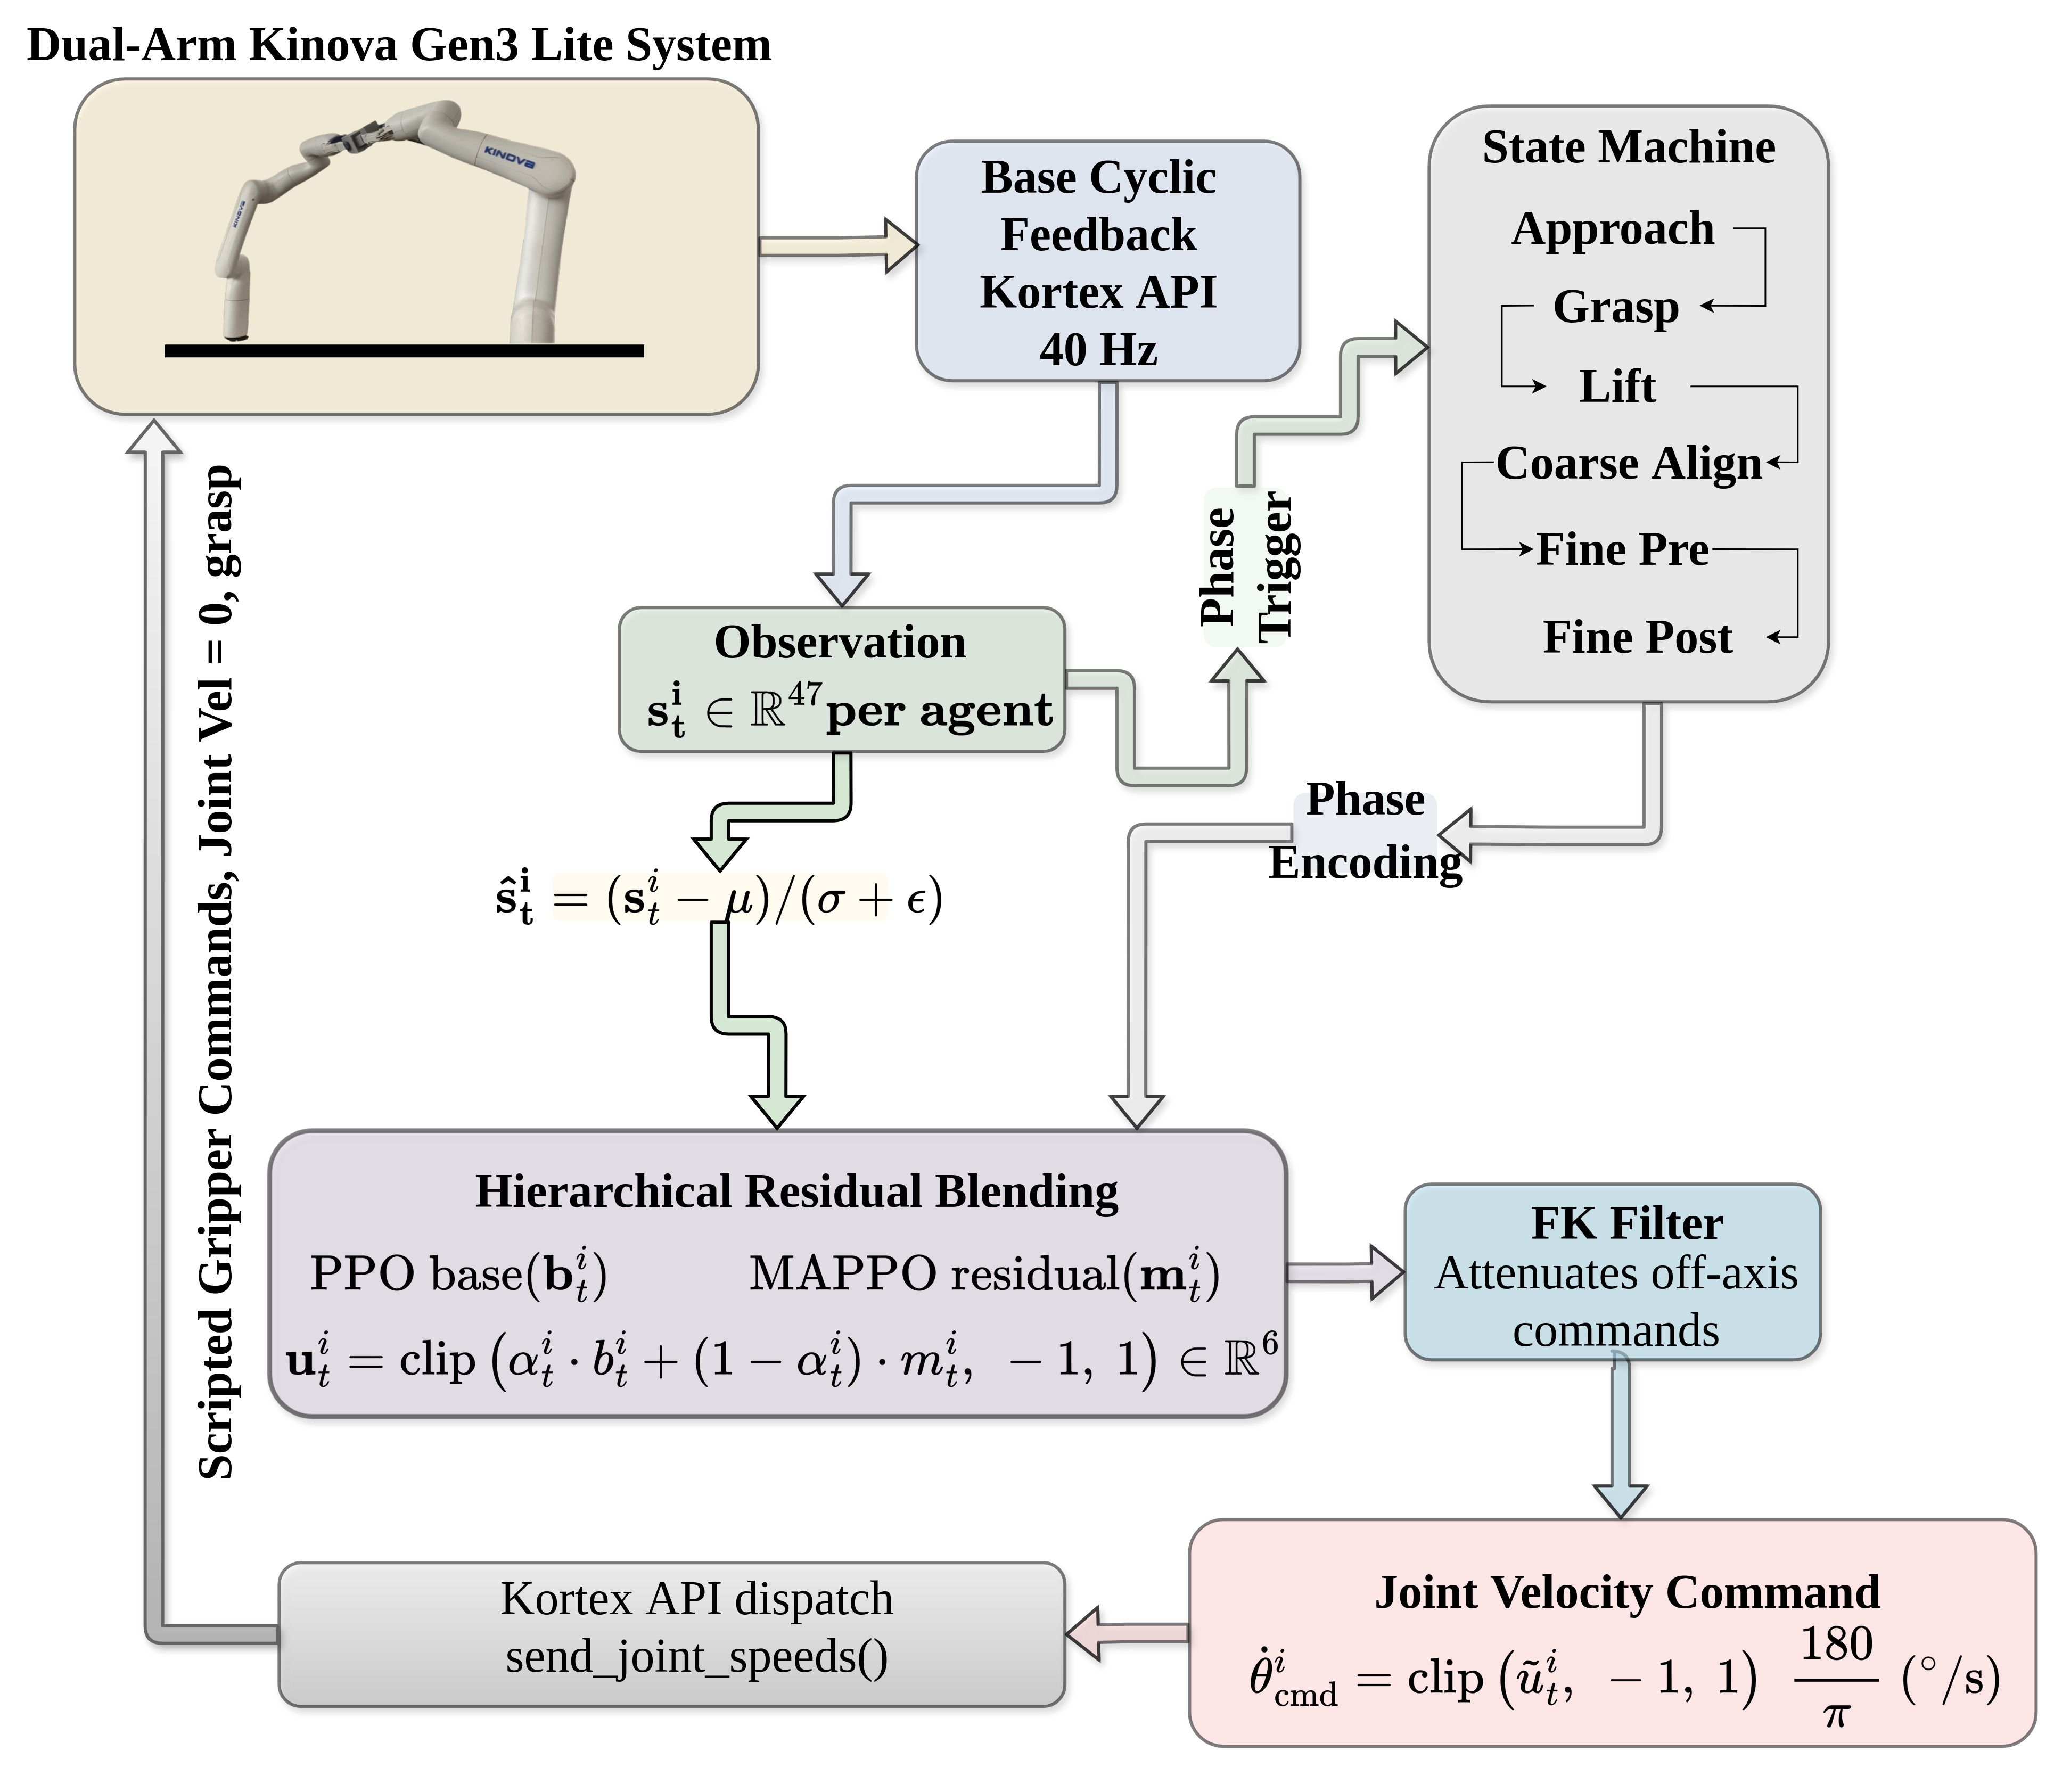
\includegraphics[width=\linewidth]{figs/Fig_2.jpg}
    \caption{Sim-to-real deployment pipeline on dual Kinova Gen3 Lite manipulators via the Kortex API. A state machine sequences approach, grasp, and coarse/fine alignment phases; at each control step the current observation is normalized and passed to the hierarchical residual blending module, which queries the frozen PPO base policy and the MAPPO residual policy and combines their outputs into a joint velocity command, attenuated by a forward-kinematics consistency filter before dispatch via the Kortex API.}
    \label{fig:sim2real}
\end{figure}

Real-hardware deployment is governed by a state-machine controller implemented via the Kinova Kortex API, spanning active phases from initial approach to fine post-alignment. Phase transitions are triggered by the simultaneous satisfaction of positional and orientational error thresholds for both manipulators. The grasping phase is the sole exception to the policy-driven execution, during this interval, a discrete gripper command is issued. All remaining joint motion across the active phases is driven entirely by the hierarchical coordination blending policy.

The frozen PPO base policy $\pi_{\theta_{\text{ppo}}}$ is queried independently per arm to produce $\mathbf{b}_t^i$, the MAPPO actor $\pi_\theta$ produces the coordination policy $\mathbf{m}_t^i$ and blending increment $\mathbf{\Delta\alpha}_{t}^{i}$, and the final blended command $\tilde{\mathbf{u}}_t^i$ is computed per Eq.~(\ref{combined_action_noise}). The blended action is then scaled and converted to hardware joint velocity commands dispatched via the Kortex API as in Eq.~(\ref{hard_ware_vel}):
\begin{equation}
\dot{\theta}_{\text{cmd}}^i =
\mathrm{clip}\left( \tilde{u}_t^i,\ -1,\ 1 \right)\cdot\frac{180}{\pi}
\; (\mathrm{^\circ/s})
\label{hard_ware_vel}
\end{equation}

The phase one-hot encoding $\mathbf{e}_{\text{phase}} = [1, 0]^\top$ is maintained throughout approach, lift, and coarse alignment, switching to $\mathbf{e}_{\text{phase}} = [0, 1]^\top$ exclusively during fine alignment phases, exactly mirroring the simulation phase encoding seen during training.

During simulation training, a RunningStandardScaler maintains online estimates of the mean $\mu \in \mathbb{R}^{47}$ and standard deviation $\sigma \in \mathbb{R}^{47}$ of each agent's local observation $s_t^i$ as shown in Eq.~(\ref{normalized_obs}). These statistics are frozen at the end of training and applied to every real-hardware observation prior to policy inference:
\begin{equation}
    \hat{s}^{i}_{t} = (s^{i}_{t} - \mu)/(\sigma + \epsilon)
    \label{normalized_obs}
\end{equation}

The simulation snap mechanism, which triggers when the two offset end-effectors come within 8~cm and 0.2~rad of each other is not transferred to hardware. Without force sensing at fingers or active collision avoidance, triggering a proximity-based snap at close range risks object-to-object or arm-to-arm collision under any misalignment. Instead, the state machine enforces alignment through three predefined spatial separation way-points, coarse alignment at 0.4~m offset end-effector separation, fine pre-alignment at 0.17~m, and fine post-alignment at 0.1~m. Progression to the next way-point occurs only after both arms simultaneously satisfy position and orientation error thresholds at the current separation distance. This staged spatial approach eliminates the need for a collision avoidance module entirely, a significant deployment simplification while preserving the alignment quality achieved through learned coordination. Further, during fine alignment phases, a forward kinematics consistency check attenuates velocity commands that deviate significantly from the desired approach axis, providing a complementary hardware safety layer without modifying the policy architecture.

\section{Experiments and Results}
\label{results_and_discussion}
All experiments were conducted using the simulation environment detailed in Sec.~\ref{simulation_setup}. Each method was evaluated over 10 independent trials, each trial comprising 4,096 individual episodes. The success rates across all environments are reported in Table~\ref{tab:sim_success}. Additionally, Fig.~\ref{fig:base_line_comparisons} illustrates the comparative performance of each method, specifically showing the accumulated mean reward over the course of training. Relative success (Rel.Succ) is defined as the conditional alignment success rate among environments that successfully completed the reach phase.

\begin{figure}
    \centering
    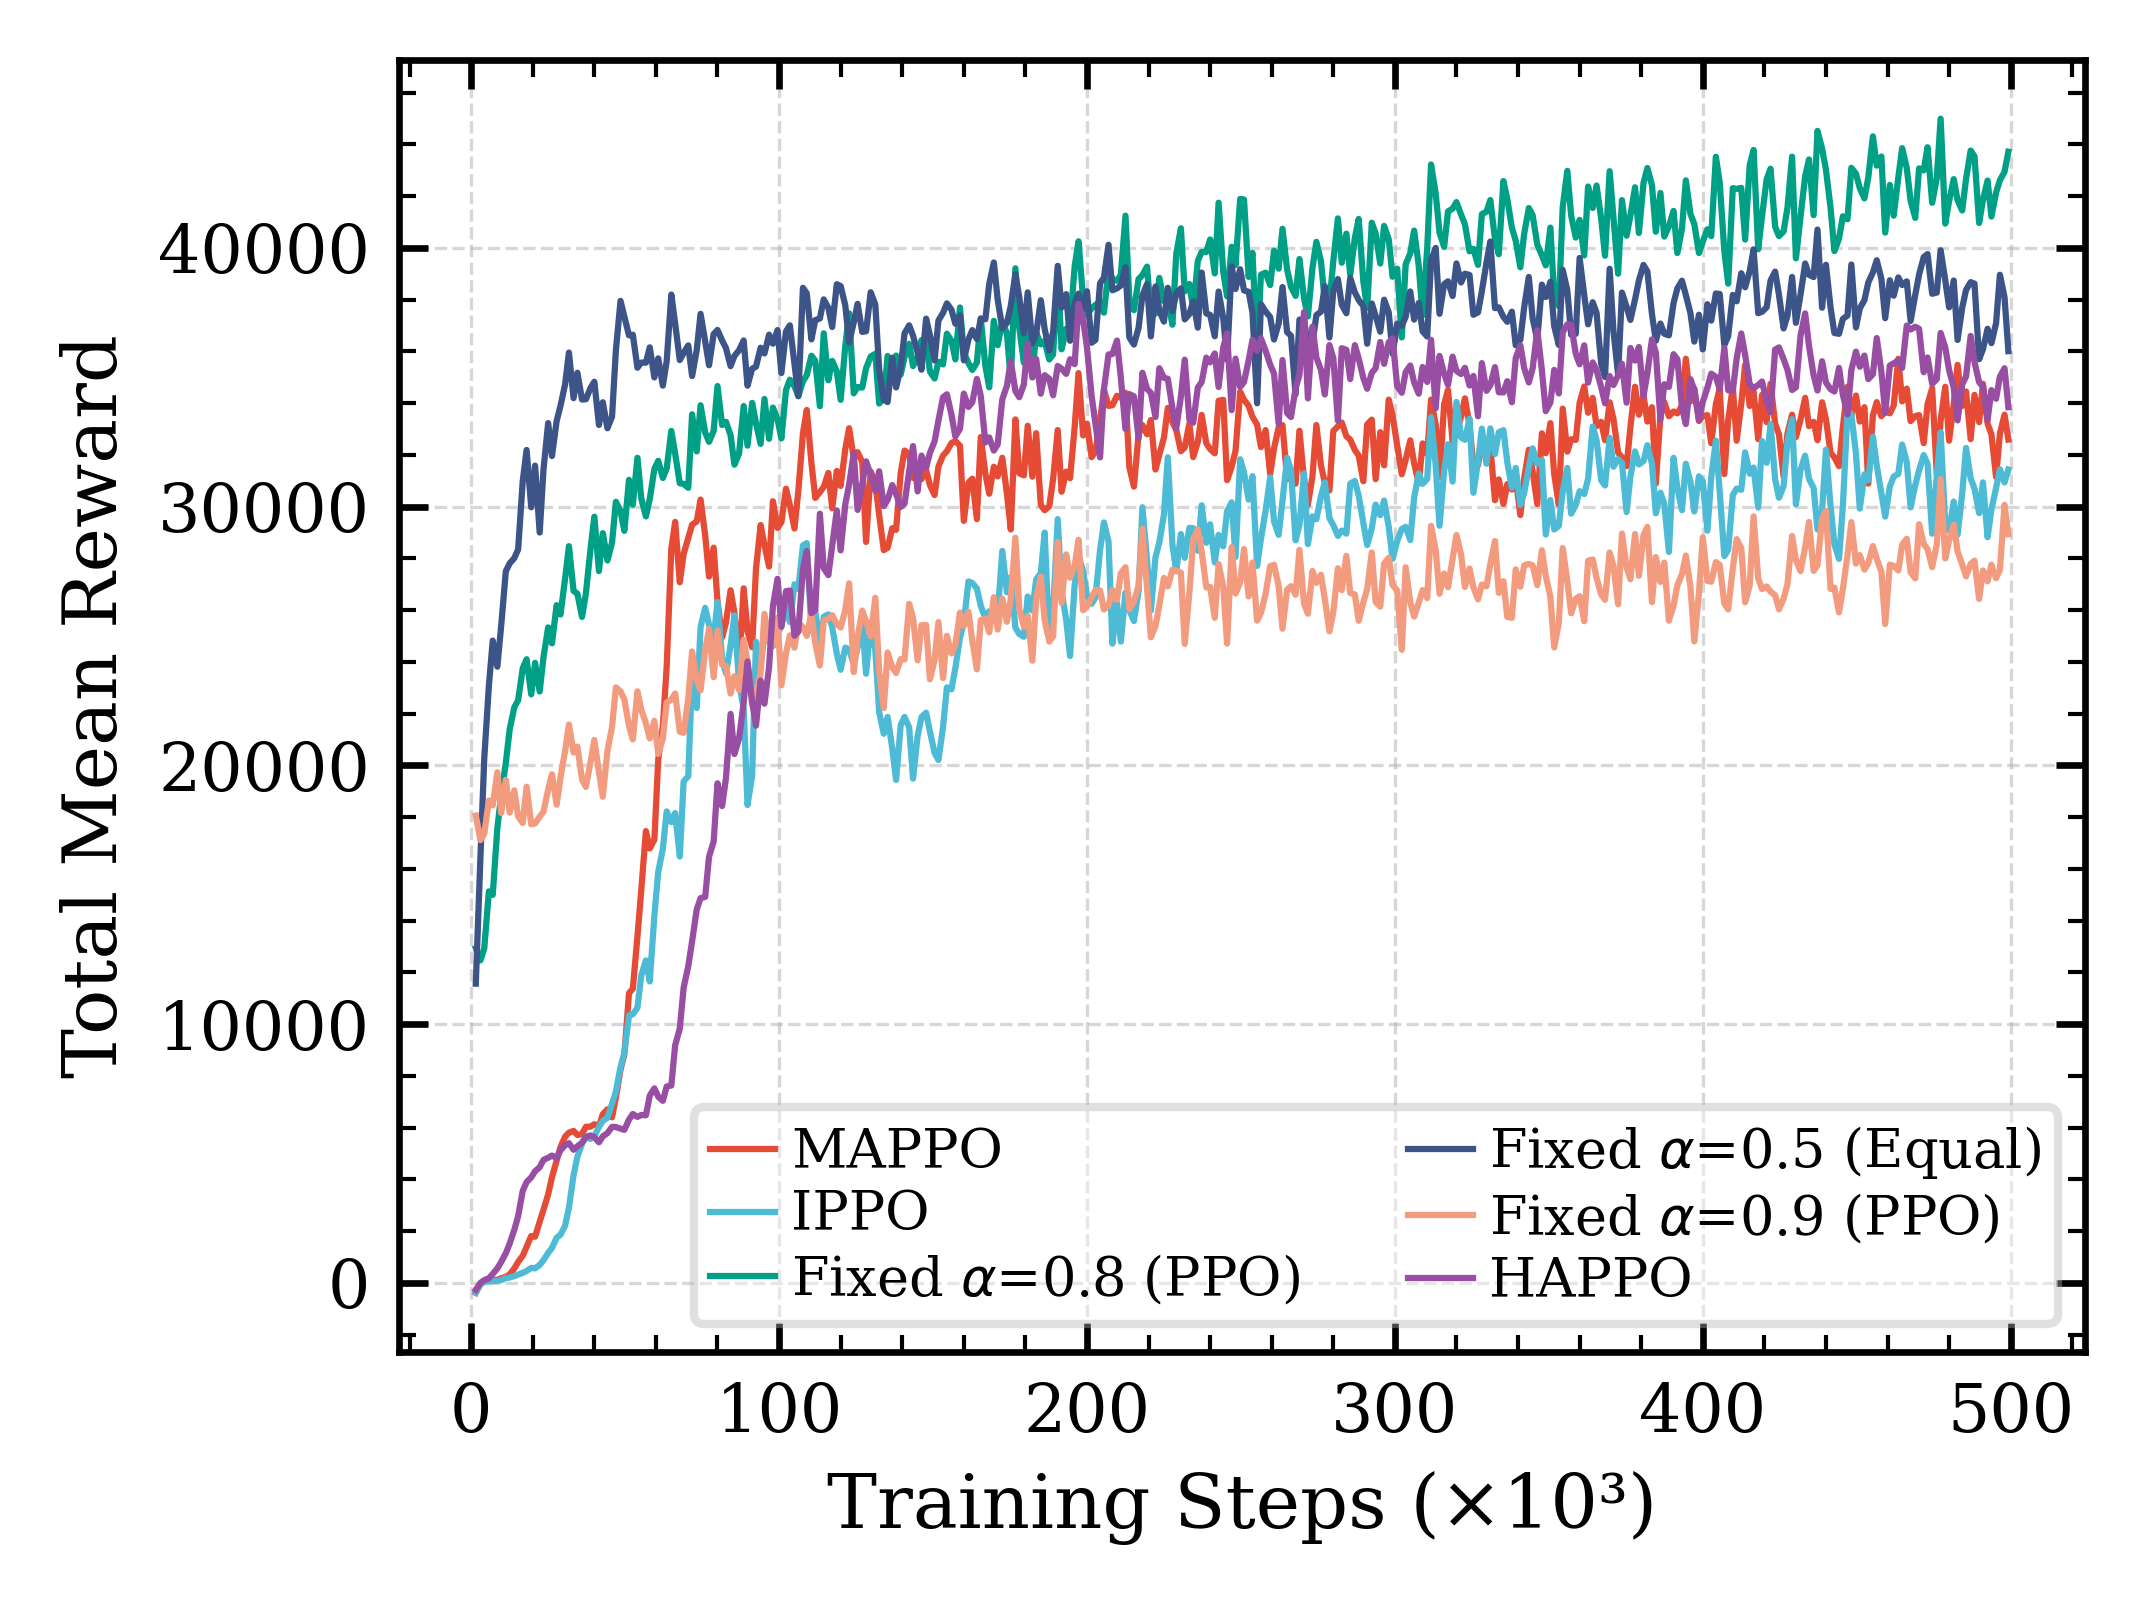
\includegraphics[width=\linewidth]{figs/Fig_3.png}
    \caption{Training reward curves for pure MARL baselines and fixed-blend PPO+MAPPO variants. Curves are Gaussian-smoothed for clarity.}
    \label{fig:base_line_comparisons}
\end{figure}

\begin{table}[h]
\caption{Baseline evaluation results over 10 trials across 4,096 parallel environments(Mean $\pm$ Std)}
\centering
\resizebox{\columnwidth}{!}{
\begin{tabular}{lccc}
\midrule 
\textbf{Method} & \textbf{Reach Succ(\%)} & \textbf{Align Succ(\%)} & \textbf{Rel.Succ(\%)} \\
\midrule \midrule
MAPPO \cite{MAPPO} & 71.6$\pm$0.5 & 8.3$\pm$0.3 & 11.6$\pm$0.5\\
HAPPO \cite{happo/htrpo} & 73.6$\pm$0.7 & 32.3$\pm$0.8 & 43.9$\pm$1.2 \\
IPPO \cite{IPPO} & 62.0$\pm$0.5& 25.0$\pm$0.3 & 40.3$\pm$0.6\\
Fixed $\alpha=0.5$ & 41.1$\pm$0.8& 18.4$\pm$0.5 & 44.8$\pm$1.1\\
Fixed $\alpha=0.8$ & 47.7$\pm$0.8& 17.6$\pm$0.8 & 36.9$\pm$1.3\\
Fixed $\alpha=0.9$ & 1.76$\pm$0.2& 0.02$\pm$0.01 & 1.1$\pm$0.6\\
\midrule
\end{tabular}}
\vspace{2pt}
    \footnotesize{\textit{Note*:}} \textit{All methods were trained under a single seed (42) and evaluated over 10 independent trials, so the reported deviations characterize evaluation variance at fixed initialization; seed-level variance for the proposed method is reported separately in Table~\ref{tab:seed_robustness}.}
\label{tab:sim_success}
\end{table}

Table~\ref{tab:sim_success} and Fig.~\ref{fig:base_line_comparisons} reveal critical performance trade-offs across all baseline configurations. Pure MAPPO achieves the highest reach success of (71.6\%), confirming that centralized training with a shared global critic enhances single-arm approach capability. However, its absolute alignment success collapses to 8.3\% with a conditional alignment rate of only 11.6\%. This exposes the fundamental sample complexity cost of learning low-level reachability and high-level cooperative alignment simultaneously from a single reward signal under joint policy optimization. In contrast, Pure IPPO achieves a higher absolute alignment success (25.0\%) and conditional alignment rate (40.3\%) despite an inferior reach rate (62.0\%). This inversion indicates that decentralized independent critics, while blind to the partner agent's state, encourage more conservative per-arm behaviors that reduce inter-agent interference during fine alignment convergence. This comes at the direct cost of coordination quality as measured by the centralized reward signal. Although, HAPPO achieves the highest reaching success among MARL baselines (73.6\%), yet its alignment success (32.3\%) and conditional success rate (43.9\%) remain well below GPC. While HAPPO retains a centralized critic with global state access, its sequential actor update scheme, the mechanism providing its monotonic improvement guarantee updates each agent's policy in turn. Consequently, the other agent's advantage is computed against a shifted joint policy. In a bilateral alignment task requiring simultaneous inter-arm convergence, this sequential actor asymmetry directly disrupts the coordinated policy updates that require strict alignment demands.

Fixed-ratio blending reveals a critical and counterintuitive reward-success decoupling. Despite achieving the highest cumulative training rewards (Fig.~\ref{fig:base_line_comparisons}), fixed ratios of $\alpha^{i}_{t}=0.8 \text{ \& }0.5$ yield reach success of 47.7\% and 41.1\% respectively, below both pure methods with absolute alignment success of 17.6\% and 18.4\%, both well below Pure IPPO (25.0\%). Critically, their conditional alignment rates of 36.9\% ($\alpha^{i}_{t}=0.8$) and 44.8\% ($\alpha^{i}_{t}=0.5$) reveal that even among environments completing reach successfully, bilateral alignment coordination remains unreliable. Notably, $\alpha^{i}_{t}=0.8$ performs worse than Pure IPPO (40.3\%) on the conditional metric despite incorporating the frozen PPO prior, demonstrating that a rigidly dominant base policy actively suppresses the MAPPO coordination's capacity to enforce inter-arm coordination. While $\alpha^{i}_{t}=0.5$ marginally exceeds Pure IPPO on the conditional metric, its substantially lower reach success (41.1\% vs. 62.0\%) indicates the equal-weight blend interferes with single-arm approach convergence. The high cumulative rewards under fixed blending are explained by the PPO prior dominating action selection throughout the episode, producing smooth single-arm trajectories that accumulate dense per-step rewards without achieving bilateral task completion. The extreme case of $\alpha^{i}_{t}=0.9$ confirms this, reach success collapses to 1.76\%, conditional alignment to 1.1\%, and absolute alignment to effectively zero (0.02\%), yet the reward curve remains among the highest across all methods. This definitively demonstrates that cumulative reward is an unreliable proxy for cooperative task success in hierarchical multi-agent systems when the base policy contribution dominates the action space.

These findings jointly motivate the two core design choices of the proposed framework. The adaptive $\alpha^{i}_{t}$ mechanism avoids the fixed-ratio regimes by allowing each agent to dynamically regulate PPO prior reliance as a function of real-time coordination demand deferring to the base policy during independent reaching and suppressing it when bilateral convergence requires coordinated deviation. 

\begin{figure}
    \centering
    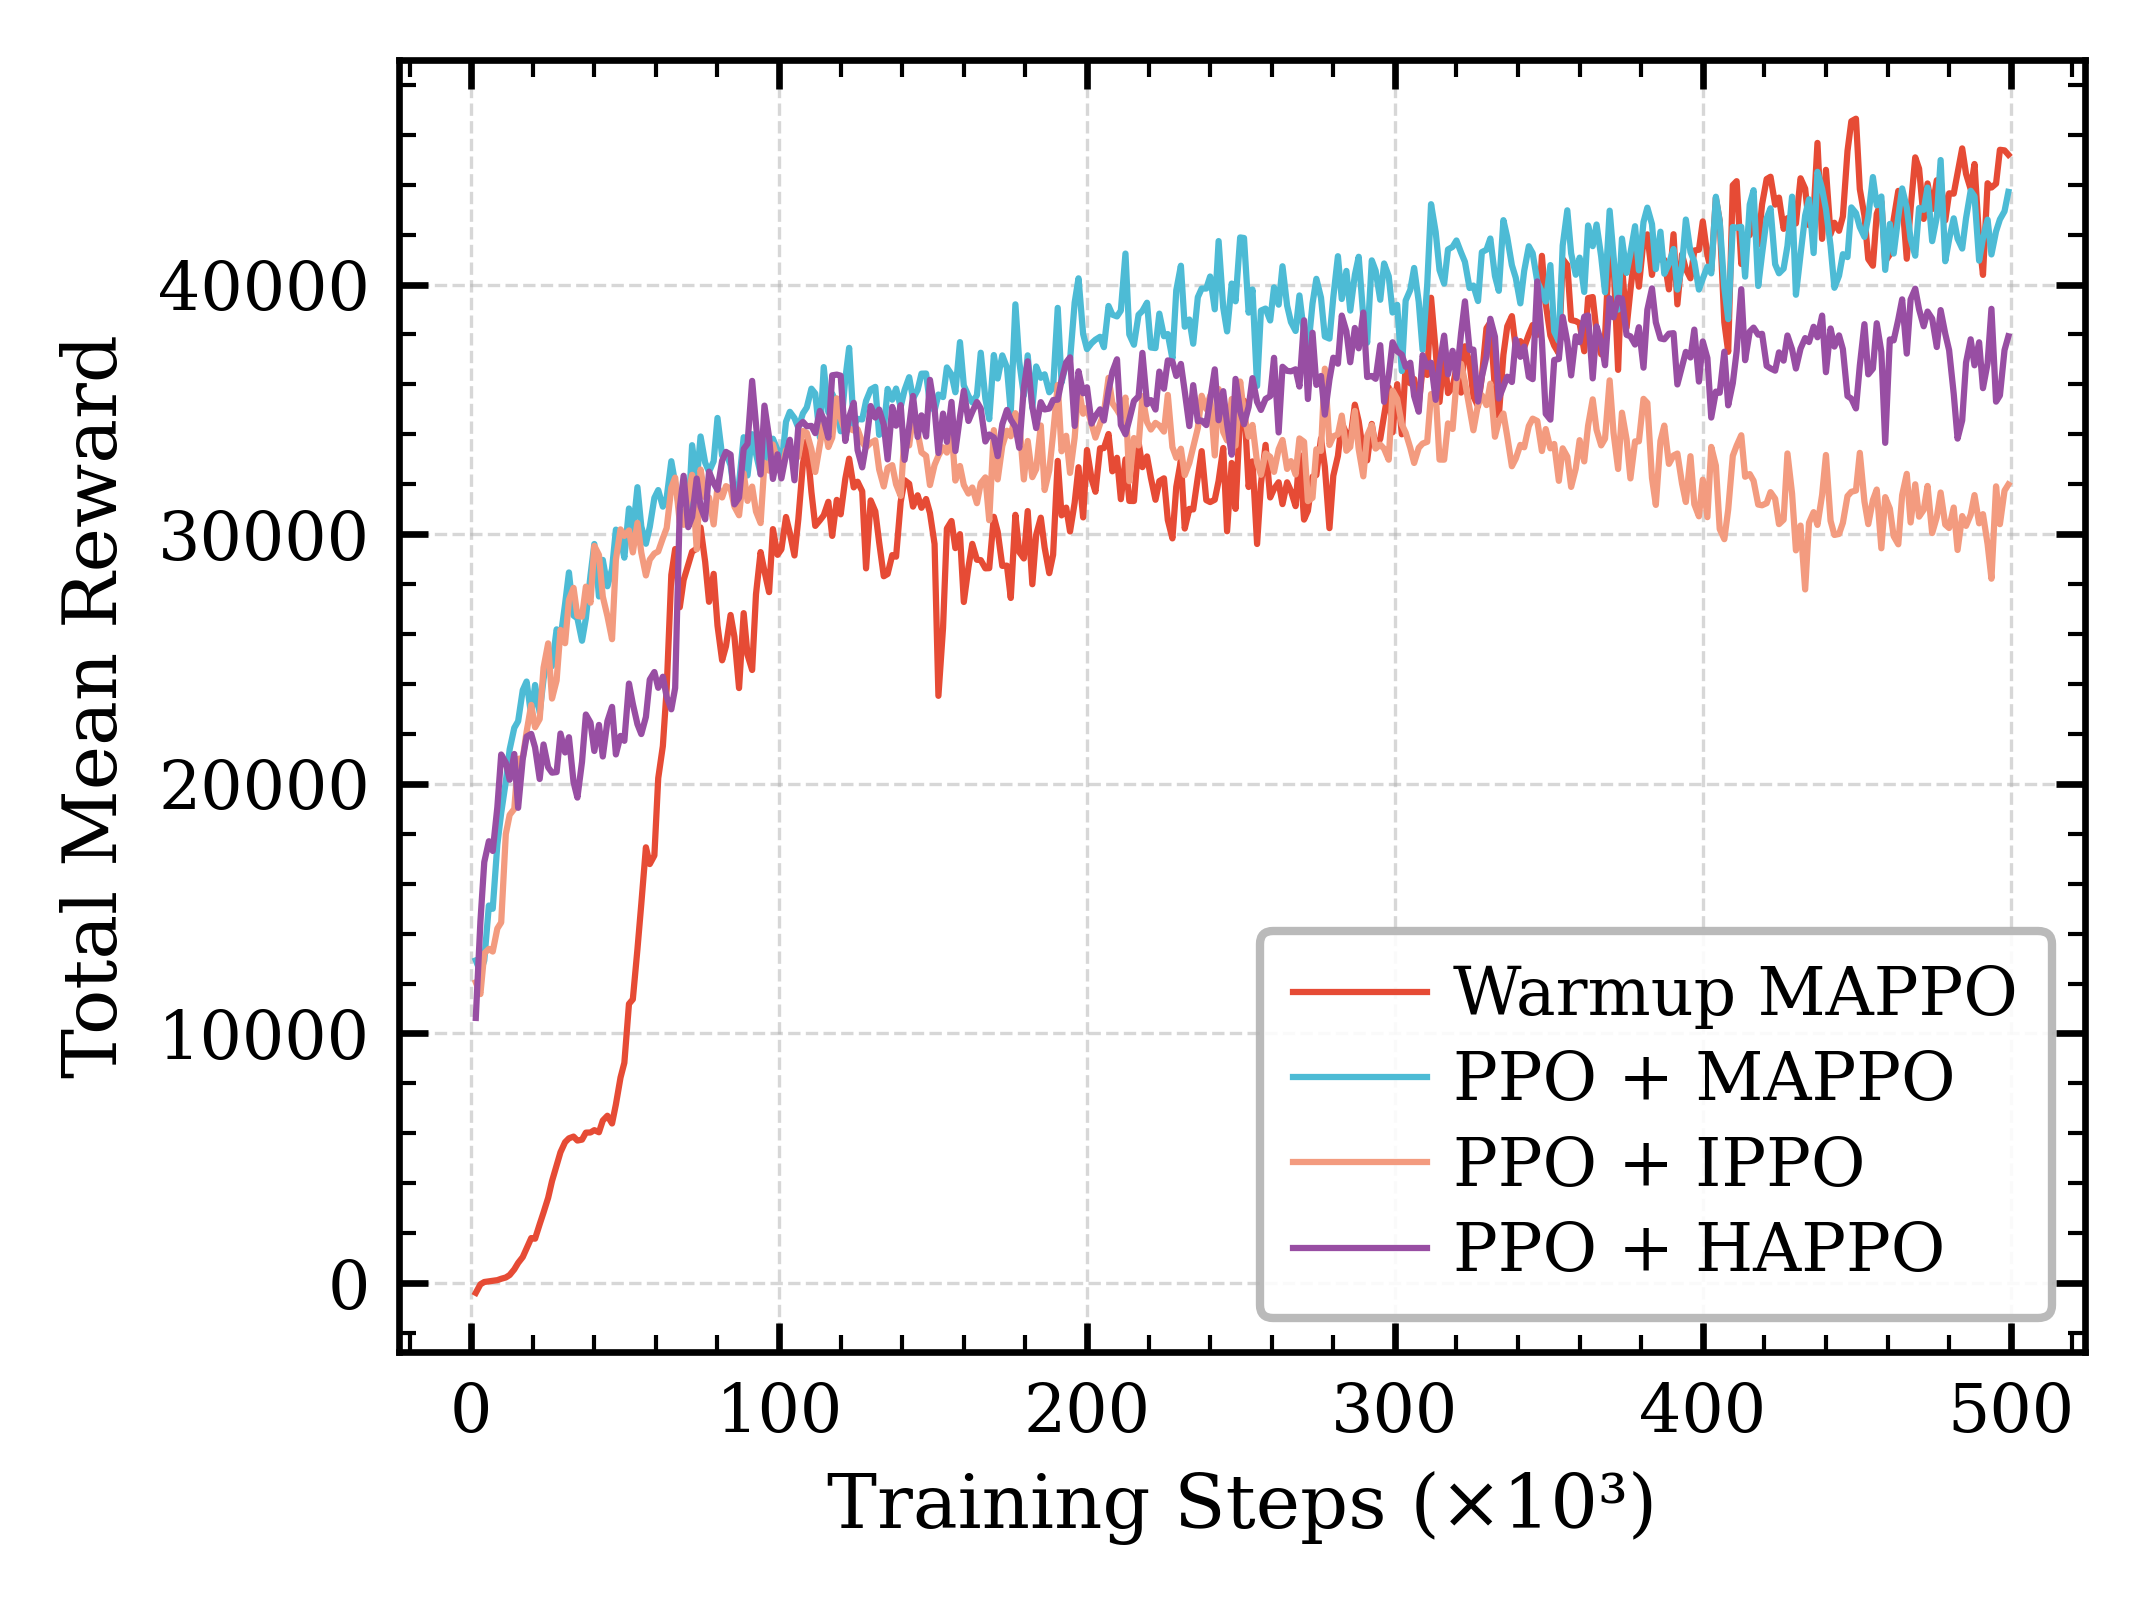
\includegraphics[width=\linewidth]{figs/Fig_4.png}
    \caption{Ablation training reward curves: adaptive blending with MARL Methods and warmup variant (150k-step scale freeze).}
    \label{fig:ablation_study}
\end{figure}
\begin{table}[h]
\caption{Ablation study results over 10 trials across 4,096 parallel environments(Mean $\pm$ Std)}
\centering
\resizebox{\columnwidth}{!}{
\begin{tabular}{lccc}
\midrule 
\textbf{Method} & \textbf{Reach Succ(\%)} & \textbf{Align Succ(\%)} & \textbf{Rel.Succ(\%)} \\
\midrule \midrule
Warmup MAPPO & 88.50$\pm$0.3& 85.80$\pm$0.2 & 96.94$\pm$0.3\\
\textbf{PPO + MAPPO (ours)} & \textbf{96.50$\pm$0.3} & \textbf{95.0$\pm$0.4} & \textbf{98.45$\pm$0.4}\\
PPO + IPPO  & 67.50$\pm$0.7& 62.50$\pm$0.9 & 92.60$\pm$1.2\\
PPO + HAPPO & 92$\pm$0.2 & 87$\pm$0.4 & 94.60$\pm$0.5\\
\midrule
\end{tabular}}
\vspace{2pt}
    \footnotesize{\textit{Note*:}} \textit{All variants were trained under a single seed (42); the reported deviations therefore characterize evaluation variance at fixed initialization. Seed-level variance for the proposed method is reported in Table~\ref{tab:seed_robustness}.}
\label{tab:ablation_metrics}
\end{table}

Table~\ref{tab:ablation_metrics} and Fig.~\ref{fig:ablation_study} illustrate the individual contributions of adaptive blending, centralized training, and the warm-up curriculum. PPO+MAPPO (Adaptive, from t=0) achieves the highest performance across all metrics (96.5\% reach, 95.0\% alignment, and 98.45\% relative success), confirming that the combination of adaptive $\alpha^{i}_{t}$ and CTDE is the optimal configuration. PPO+IPPO (Adaptive), despite employing the same adaptive blending mechanism, yields substantially lower success in reaching (67.5\%), alignment (62.5\%), and relative success (92.59\%). This result directly demonstrates that the centralized critic is not redundant, without global state access during training, the decentralized coordination  policy cannot learn the precise bilateral coordination required for alignment convergence. The 32.5\% alignment gap and 5.86\% relative success gap between PPO+IPPO and PPO+MAPPO successfully isolates the contribution of CTDE independently of the blending mechanism. PPO+HAPPO (Adaptive) achieves 92\% reach and 87\% alignment with stable reward convergence. Both HAPPO and MAPPO condition their critics on the identical 92-D global state; the two differ only in the actor update. HAPPO updates the agents sequentially, reweighting the second agent's advantage by the importance ratio of the first, whereas MAPPO updates both simultaneously. The residual 8-point alignment gap at this seed therefore isolates the cost of sequential factored updates in a task demanding simultaneous bilateral convergence, rather than any difference in critic observability.

The Warmup MAPPO variant, which freezes $\alpha^{i}_{t}$ at zero for the first 150k timesteps before enabling adaptive blending, achieves 88.5\% reach, 85.8\% alignment, and 96.94\% relative success. While competent, it underperforms PPO+MAPPO (Adaptive) by approximately 9\% on reach and alignment, and 1.5\% on relative success. Its reward curve, shown in Fig.~\ref{fig:ablation_study}, exhibits a pronounced dip and delayed recovery around the 150k transition point, indicating that the abrupt introduction of blending after a pure MAPPO warmup disrupts the established policy. In contrast, PPO+MAPPO (Adaptive) enables blending from the initial timestep, allowing the policy to co-adapt the coordination policy and the blending gate jointly from the outset.

\begin{table}[h]
\caption{Seed robustness of PPO+MAPPO (Adaptive) and of the $\alpha$-detached control. Each seed evaluated over 10 independent trials across 4,096 parallel environments (Mean $\pm$ Std across trials). Each block's final row reports Mean $\pm$ Std across the three training seeds.}
\centering
\resizebox{\columnwidth}{!}{
\begin{tabular}{lccc}
\midrule
\textbf{Training Seed} & \textbf{Reach Succ(\%)} & \textbf{Align Succ(\%)} & \textbf{Rel.Succ(\%)} \\
\midrule \midrule
42  & 96.54$\pm$0.37 & 95.07$\pm$0.49 & 98.47$\pm$0.21 \\
100 & 95.81$\pm$0.29 & 93.48$\pm$0.42 & 97.57$\pm$0.27 \\
200 & 95.40$\pm$0.49 & 93.03$\pm$0.42 & 97.52$\pm$0.18 \\
\midrule
\textbf{Across seeds} & \textbf{95.92$\pm$0.58} & \textbf{93.86$\pm$1.07} & \textbf{97.86$\pm$0.53} \\
\midrule \midrule
\multicolumn{4}{l}{\textit{PPO+MAPPO ($\alpha$-detached)}} \\
\midrule
42  & 81.80$\pm$0.62 & 49.86$\pm$0.56 & 60.96$\pm$0.92 \\
100 & 81.74$\pm$0.50 & 59.78$\pm$0.55 & 73.13$\pm$0.86 \\
200 & 81.47$\pm$0.74 & 69.24$\pm$0.87 & 84.99$\pm$0.54 \\
\midrule
\textbf{Across seeds} & \textbf{81.67$\pm$0.18} & \textbf{59.62$\pm$9.69} & \textbf{73.03$\pm$12.02} \\
\midrule
\end{tabular}}
\label{tab:seed_robustness}
\end{table}

GPC was trained under three independent seeds (42, 100, 200), each evaluated with the protocol used for all other methods (Table~\ref{tab:seed_robustness}). Across seeds, GPC attains 95.92$\pm$0.58\% reach, 93.86$\pm$1.07\% alignment, and 97.86$\pm$0.53\% relative success. The across-seed deviation exceeds the within-seed evaluation deviation on every metric (1.07\% vs. 0.42--0.49\% on alignment), isolating initialization as a small but measurable variance component. Relative success varies least, by 0.95\% against 1.14\% and 2.04\% for reach and alignment, localizing seed sensitivity to the approach phase and indicating that the learned coordination behavior is near initialization-invariant. The 6.9-point alignment margin over PPO+HAPPO (Adaptive) spans approximately six across-seed deviations and is therefore not attributable to seed variation.

To isolate whether this margin reflects the \emph{learned} value of $\alpha^{i}_{t}$, or is merely a consequence of the seventh output dimension enlarging the action space and altering training dynamics, an $\alpha$-detached control was trained. Architecture, hyperparameters, and training budget are identical to PPO+MAPPO (Adaptive), with a gradient mask applied at the output layer and $\log\sigma$ parameters corresponding to dimension 6. Under this mask, $\alpha^{i}_{t}$ continues to be emitted per-state and to enter the blend, the log-probability, the importance ratio, and the KL term used by the learning-rate scheduler, but it never receives an update from the task objective. Trained under the same three seeds and evaluated with the identical protocol (Table~\ref{tab:seed_robustness}), the detached control attains 81.67$\pm$0.18\% reach, 59.62$\pm$9.69\% alignment, and 73.03$\pm$12.02\% relative success, a 34.2-point alignment deficit against the adaptive variant. Reach success is comparable to the fixed-ratio baselines (Table~\ref{tab:ablation_metrics}) and shows seed variance on par with the adaptive method (0.18\% vs. 0.58\%), consistent with the frozen prior alone driving single-arm approach regardless of the gating head's training status. Alignment success, by contrast, exhibits a 9.69\% across-seed deviation, roughly nine times the adaptive variant's 1.07\%, indicating that whether the untrained head's fixed random projection happens to route the blend favorably during the coordination phase is left to initialization rather than resolved by learning. This asymmetry, tight reach variance paired with wide alignment variance, localizes the cost of an untrained $\alpha^{i}_{t}$ specifically to the phase requiring active suppression of the prior. It is itself evidence against the extra-capacity explanation: were the gain attributable to the added output dimension independent of its training, the detached control would be expected to track the adaptive variant's stability on both metrics, rather than diverge sharply on one.

\begin{figure}
    \centering
    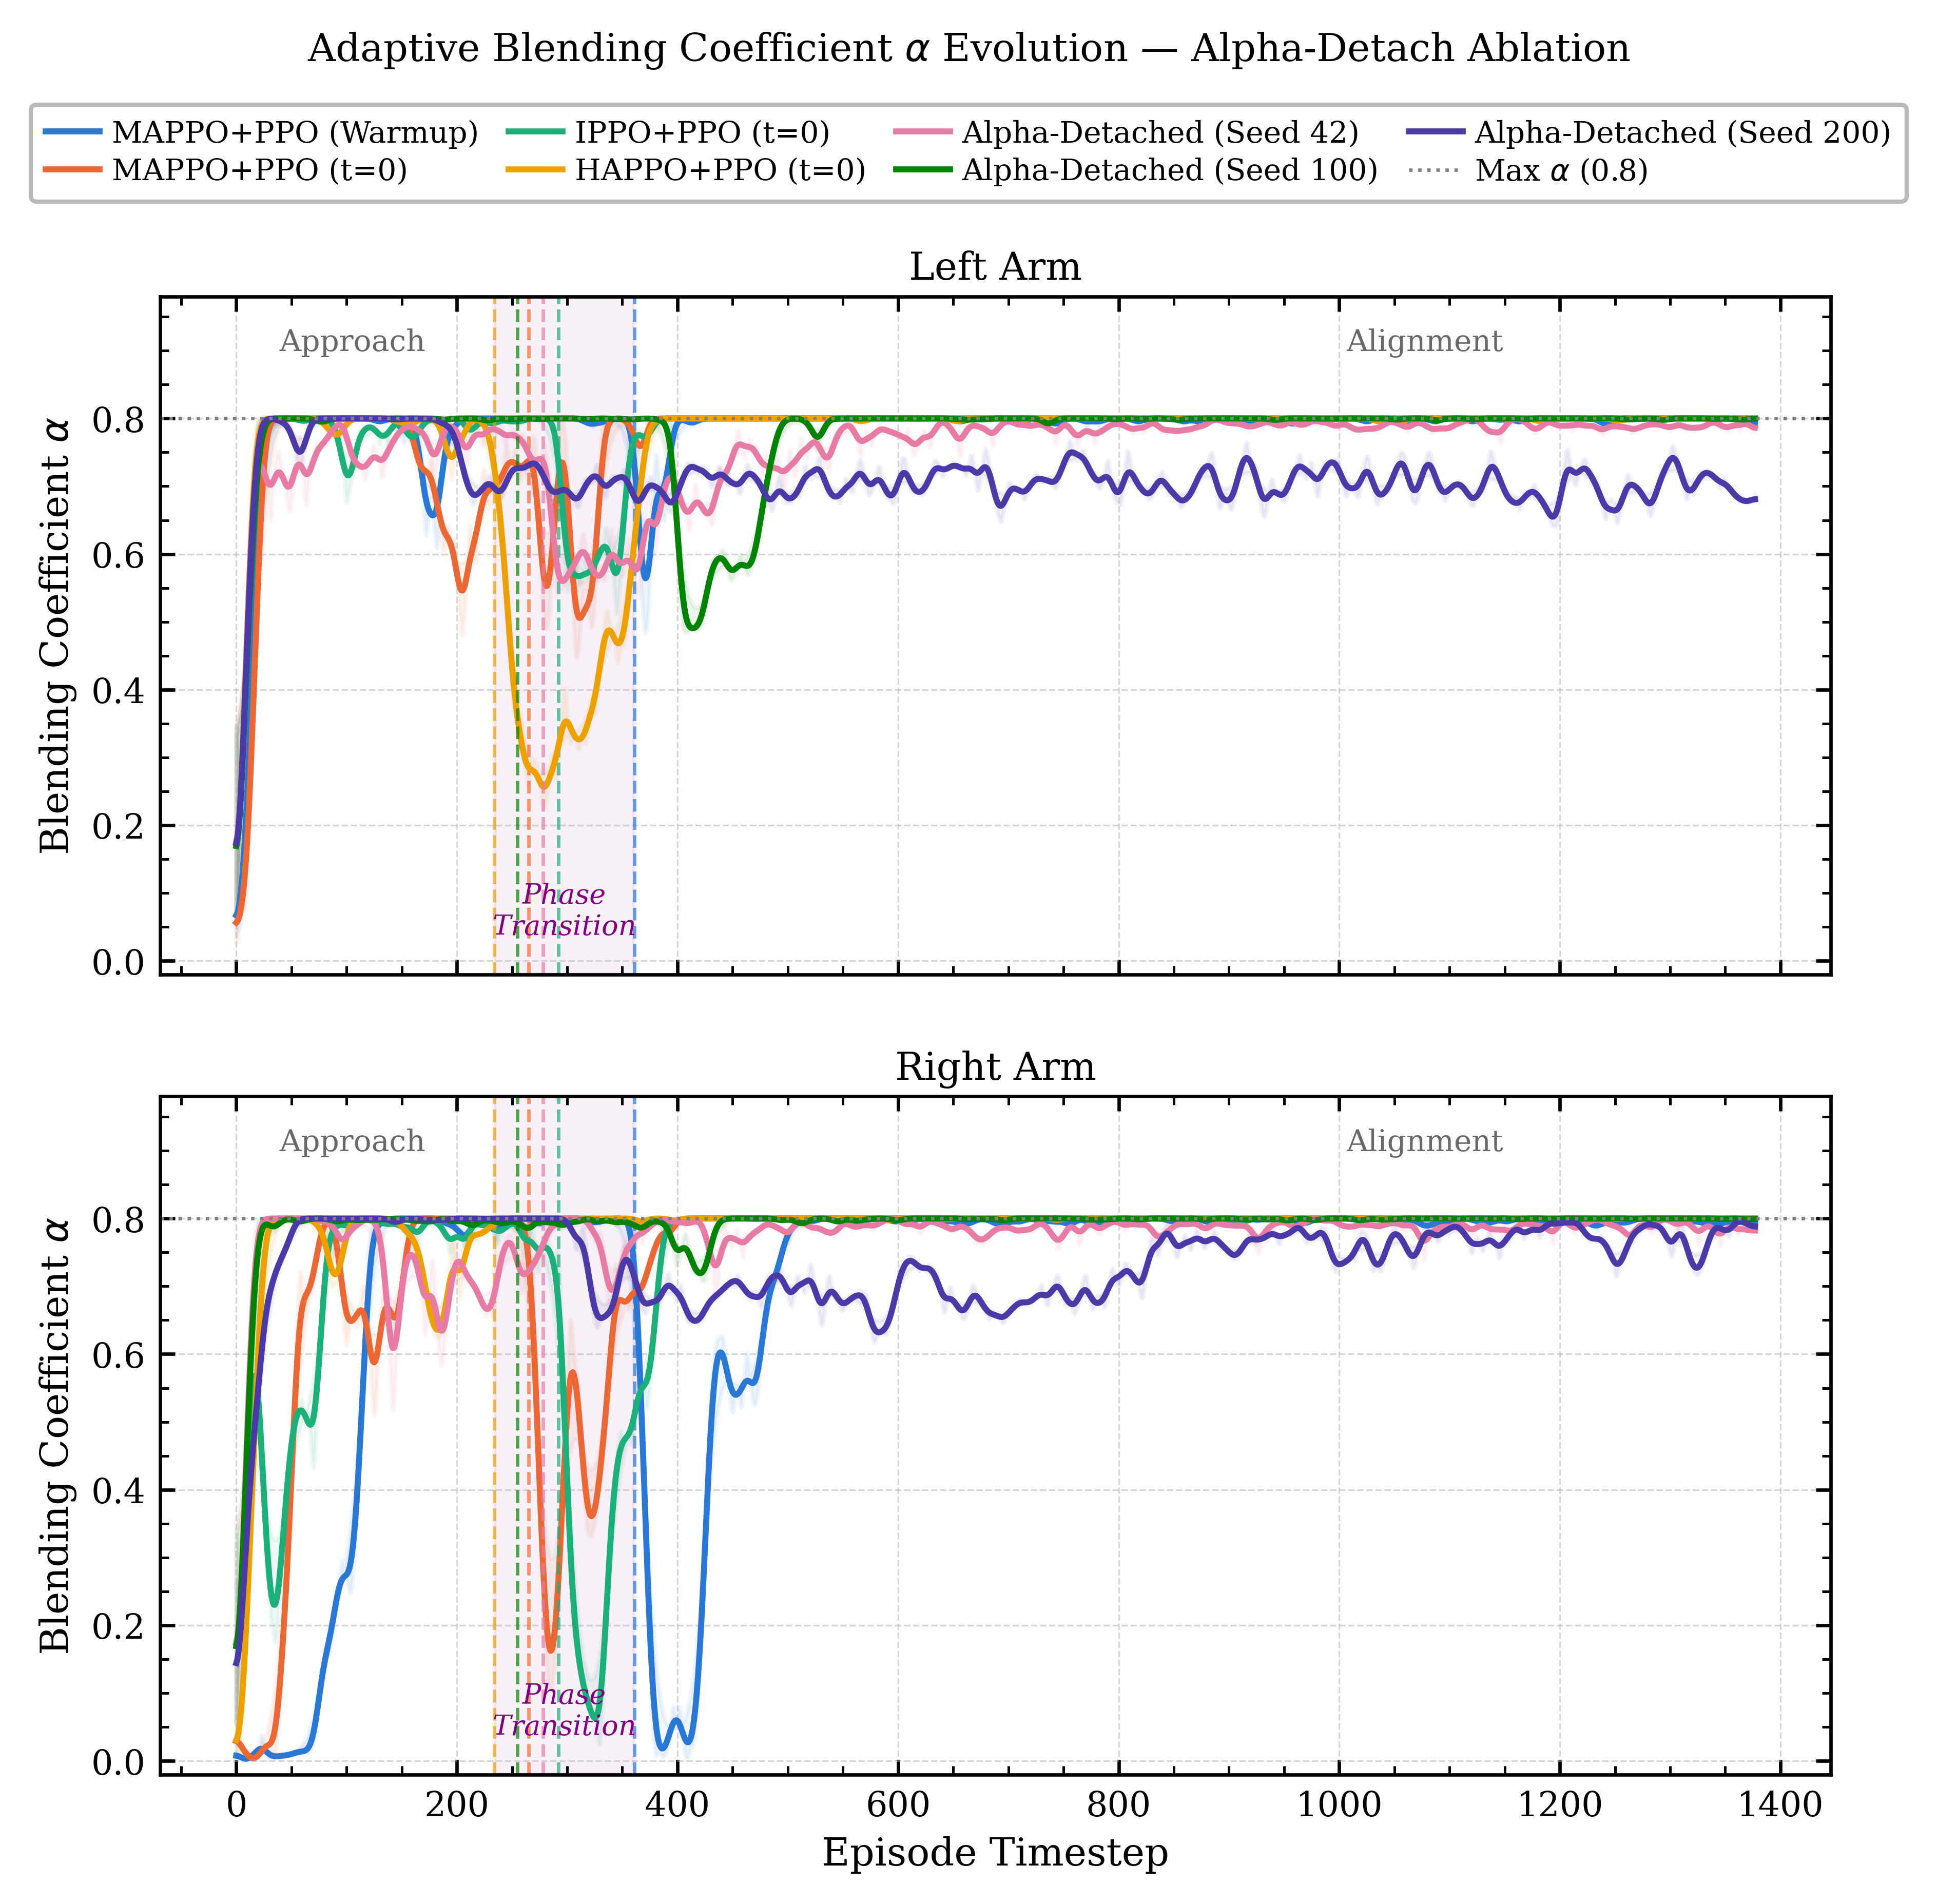
\includegraphics[width=\linewidth]{figs/Fig_5.png}
    \caption{Adaptive blending coefficient $\alpha^i_t$ evolution over a single episode for both arms across all trained variants, alongside the $\alpha$-detached control under each of its three training seeds.}
    \label{fig:alpha_evolution}
\end{figure}

Furthermore, Fig.~\ref{fig:alpha_evolution} shows $\mathbf{\alpha}^{i}_{t}$ evolution across a single episode for both arms. During approach, all methods rapidly saturate $\mathbf{\alpha}^{i}_{t}$ to 0.8, confirming the policy learns to maximally defer to the PPO prior for single-arm reaching. At the phase transition, all methods exhibit a pronounced $\mathbf{\alpha}^{i}_{t}$ reduction; the policy actively suppresses PPO reliance when cooperative alignment demands increase and independent reaching targets become counterproductive. The $\alpha$-detached control reproduces a comparable dip at the same transition. This is because a fixed linear readout of a continuously-trained trunk responds to the abrupt change in observation statistics regardless of whether that readout was ever optimized; the dip's presence alone is therefore not sufficient evidence of learned suppression. Across its three training seeds, the $\alpha$-detached control's post-transition trajectory is inconsistent. Seeds 42 and 200 settle into a wide, noisy band (approximately 0.65--0.75) that does not return to the adaptive plateau, while seed 100 recovers to a trajectory visually similar to the trained variants (Fig.~\ref{fig:alpha_evolution}). This last case is informative precisely because it dissociates trajectory shape from task outcome: despite reaching an $\alpha^{i}_{t}$ profile resembling the adaptive method, seed 100 attains only 59.78\% alignment success against the adaptive variant's 93.86\% (Table~\ref{tab:seed_robustness}), a 34-point deficit. Reaching a plausible $\alpha^{i}_{t}$ value is therefore not sufficient for coordinated task success. Under the detached control, the trunk continues training on dimensions 0--5 while dimension 6 remains a fixed random readout of that evolving representation, so any resemblance to the adaptive trajectory arises without the gating update and the coordination update ever being shaped by the same gradient. This co-adaptation, not the specific value $\alpha^{i}_{t}$ settles at, is the empirical basis for the adaptive blending mechanism: an untrained gating head, whether or not its trajectory happens to resemble the trained one, leaves the coordination policy without a blending signal that has been optimized jointly with it.

The asymmetric dip depth and recovery timing between the left and right arms across all methods reflects the structural asymmetry in their observation spaces. The left arm observes its own errors in its own frame while receiving the right arm's errors transformed into the left frame, and vice versa for the right arm. This produces distinct error magnitudes and gradient signals at the phase transition even under identical task conditions. This per-agent asymmetry is a direct consequence of the decentralized execution structure under CTDE, where each actor conditions on a locally-framed 47-D observation rather than a 92-D shared global representation. PPO+MAPPO (Ours) shows the shallowest and shortest dip on both arms, recovering fastest due to the centralized critic's global coordination signal. PPO+IPPO exhibits a deeper, oscillatory dip; decentralized critics cannot resolve the coupled bilateral alignment without global state access, and the asymmetry is more pronounced as each arm independently attempts to re-establish its gating strategy without awareness of the other's blending state. Warmup MAPPO shows a prolonged depression with delayed right-arm recovery, consistent with the reward instability in Fig.~\ref{fig:ablation_study}: abrupt blending introduction after the 150K freeze disrupts co-adapted gating and coordination behaviors, and the right arm recovers more slowly due to its geometrically distinct workspace position relative to the alignment convergence point. PPO+HAPPO exhibits the deepest dip across both arms at phase transition, reflecting maximum uncertainty in prior reliance when bilateral coordination is demanded without global state access. The $\alpha$-detached control's post-transition behavior is seed-dependent rather than consistently unresolved, yet alignment success remains far below the adaptive variant on every seed, including the one whose trajectory most resembles it. This dissociation between trajectory appearance and task outcome, together with the 9.69\% across-seed deviation on alignment success against 1.07\% for the adaptive variant (Table~\ref{tab:seed_robustness}), indicates that an untrained gating head leaves alignment outcome dependent on initialization rather than on a policy jointly shaped with the coordination update.


Furthermore, real-time hardware experiments were conducted on two kinova gen3 lite manipulators, for collaborative dual-arm pick and alignment task of square and cylinder peg insertion in hole. 
\begin{figure*}
    \centering
    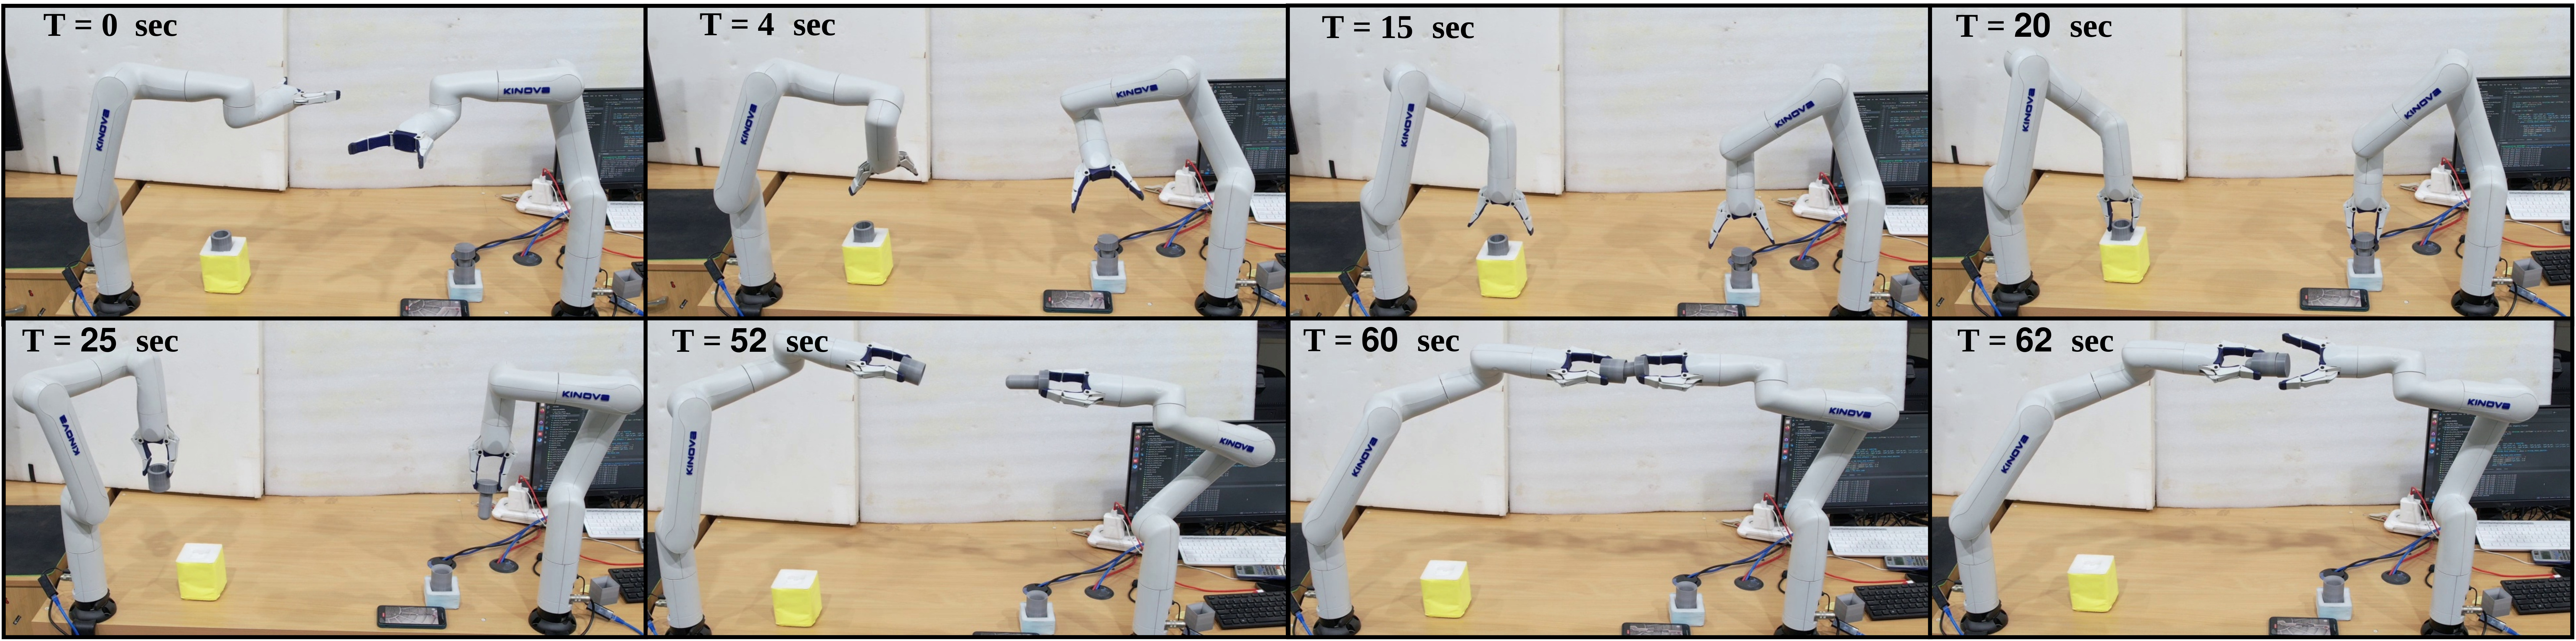
\includegraphics[width=0.9\linewidth]{figs/Fig_6.jpg}
    \caption{Sequential real-hardware execution of dual-arm pick-and-pre-assembly alignment for the cylindrical peg-in-hole task on Kinova Gen3 Lite manipulators.}
    \label{fig:real_time_exp_1_sequential}
\end{figure*}
\begin{figure*}
    \centering
    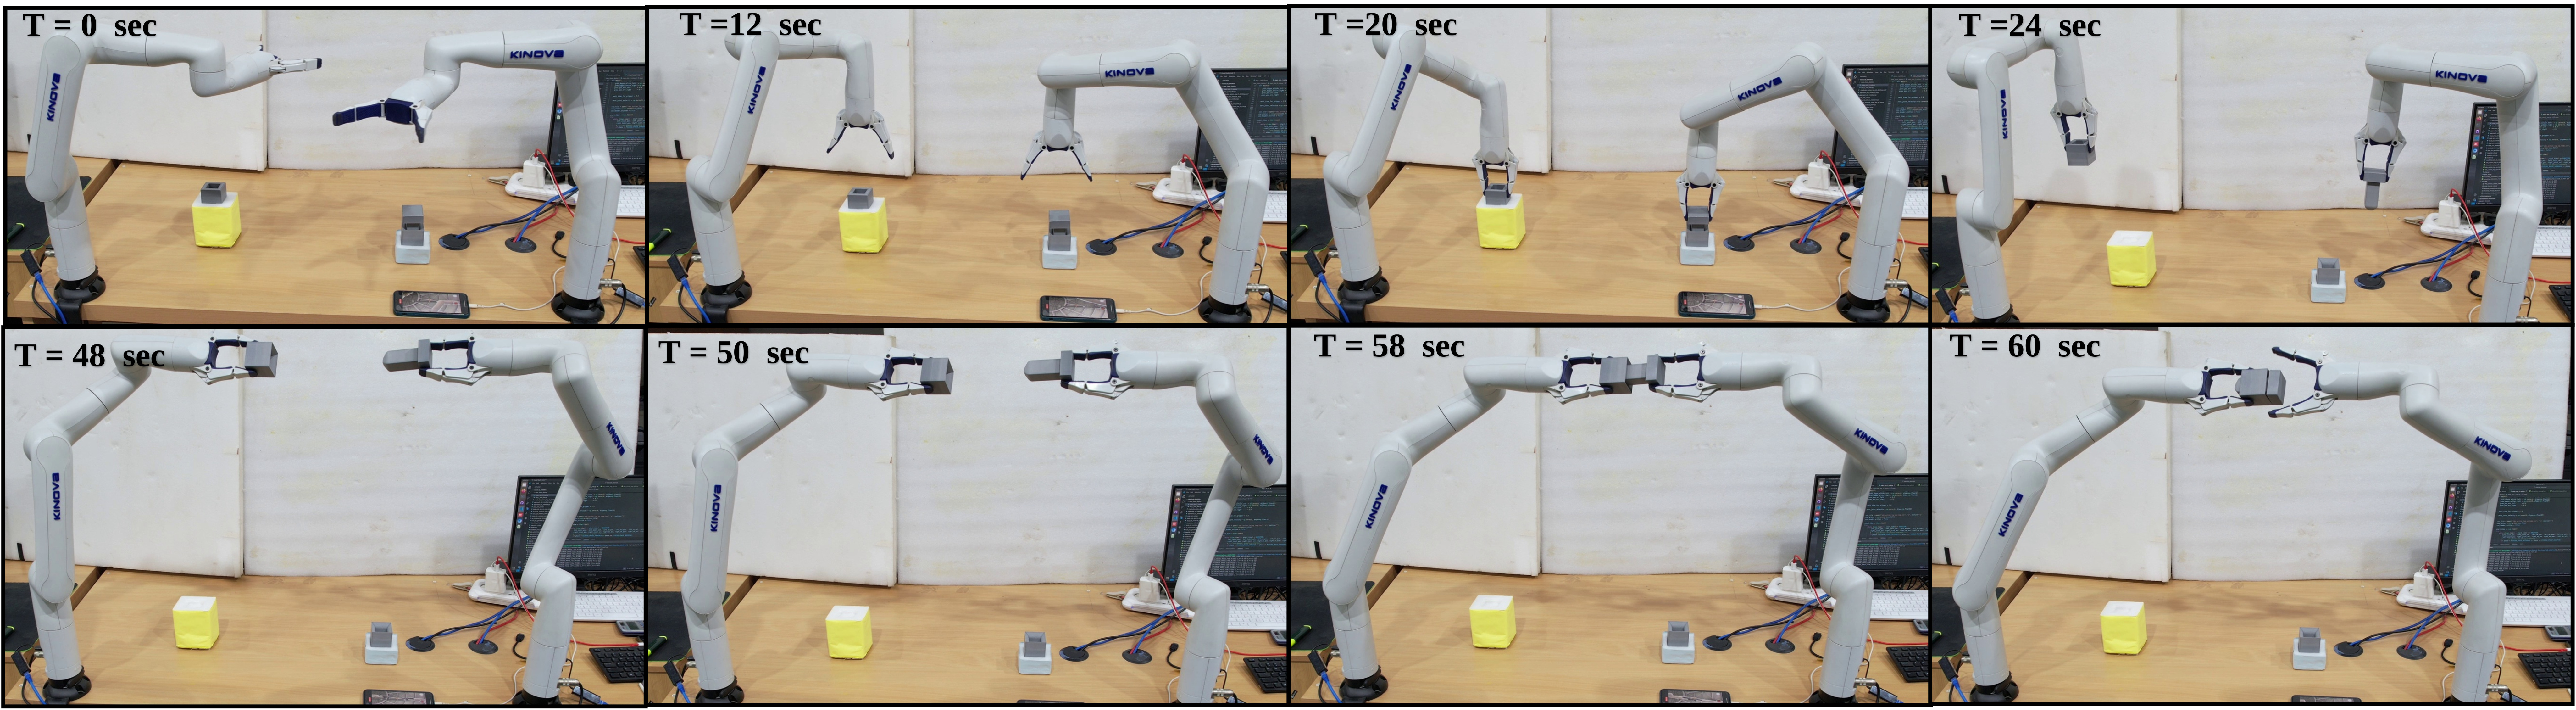
\includegraphics[width=0.9\linewidth]{figs/Fig_7.jpg}
    \caption{Sequential real-hardware execution of dual-arm pick-and-pre-assembly alignment for the square peg-in-hole task on Kinova Gen3 Lite manipulators.}
    \label{fig:real_time_exp_2_sequential}
\end{figure*}
\begin{figure*}
    \centering
    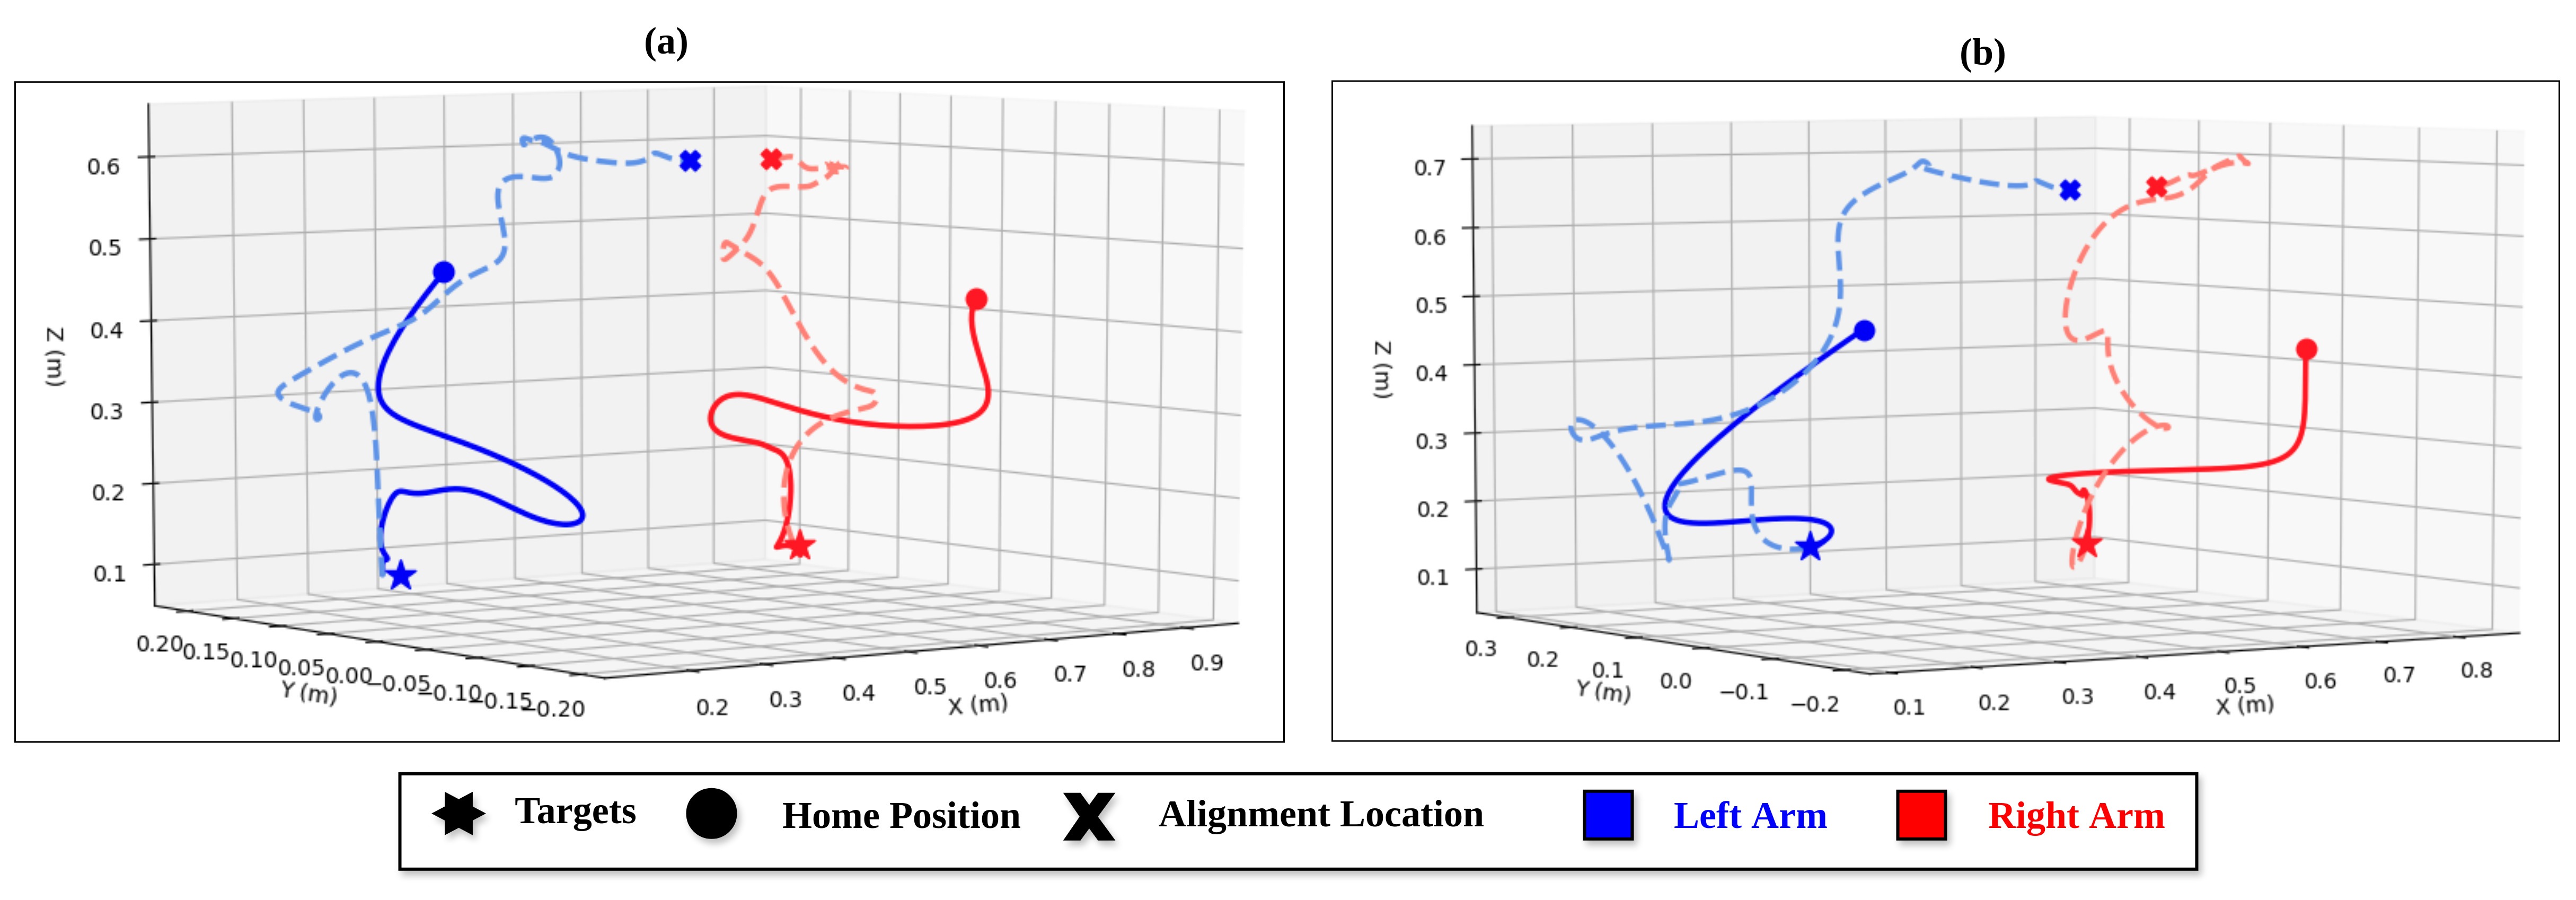
\includegraphics[width=0.9\linewidth]{figs/Fig_8.jpg}
    \caption{End-effector Cartesian trajectories during real-hardware experiments: (a) cylindrical peg-in-hole and (b) square peg-in-hole.}
    \label{fig:real_time_exp}
\end{figure*}

The experimental setup consists of a cylindrical peg and a corresponding hole positioned within the reachable workspace of the dual-arm manipulator system, as illustrated in Fig.~\ref{fig:real_time_exp_1_sequential}. The arms begin from their respective home positions (T=0~s) and reach their targets by T=4~s. Following the simultaneous convergence of positional and orientational error thresholds in the X and Y directions, while maintaining a safe Z-offset from the targets at T=15~s, the arms descend vertically to grasp the objects at T=20~s. Subsequently, the manipulators move to a safe spatial clearance to prevent potential collisions at T=25~s, eventually reaching pre-docking positions at T=52~s. Finally, through collaborative axial alignment, the objects are successfully docked by T=60~s. A similar progression is observed for the second case in Fig.~\ref{fig:real_time_exp_2_sequential}. The corresponding end-effector trajectories for both cases are provided in Fig.~\ref{fig:real_time_exp}(a) and Fig.~\ref{fig:real_time_exp}(b), respectively.

\begin{table}[t]
\caption{Hardware deployment results over 30 trials with varied target positions.}
\label{hardware_result}
\centering
\footnotesize
\setlength{\tabcolsep}{4pt}
\renewcommand{\arraystretch}{1.2}
\begin{tabular}{l c c c}
\toprule
\textbf{Outcome} & \textbf{Reach} & \textbf{Align} & \textbf{Count} \\
\midrule
Successful execution            & $\checkmark$ & $\checkmark$ & 27 \\
Object slipped during insertion & $\checkmark$ & $\times$     & 1  \\
Gripper fault during grasping   & $\times$     & $\times$     & 2  \\
\midrule
\textbf{Success Rate} & \textbf{93.3\%} & \textbf{90.0\%}\textsuperscript{*} & \textbf{30} \\
\bottomrule
\end{tabular}

\vspace{2pt}
\footnotesize{\textit{Note*:}} \textit{Alignment success rate computed over all 30 trials. Relative alignment success over successful reach trials is 96.4\%. 95\% Wilson confidence intervals: Reach [78.7\%, 98.2\%], Alignment [74.4\%, 96.5\%].}
\end{table}

\section{Discussion}
\label{discussion}
The GPC framework hierarchically composes a frozen single-arm reaching prior with a MAPPO coordination policy through adaptive gating scalar $\mathbf{\alpha}^{i}_{t}$, allowing the blending mechanism and coordination policy to co-evolve from timestep zero. The centralized 92-D critic provides the bilateral coordination signal that neither fixed-blend variants nor decentralized IPPO critics can replicate. The reward-success decoupling at $\mathbf{\alpha}^{i}_{t}=0.9$ further demonstrates that dense reward accumulation is an unreliable proxy for cooperative task completion in hierarchical MARL, a finding with implications beyond this architecture.

\noindent\textbf{Hardware Constraints:} The Kinova Gen3 Lite's non-spherical, force-sensorless gripper limits grasp verification to proximity thresholds; any in-hand slip propagates as an unobservable error into alignment. The min-operator bottleneck in (Eq.~\ref{pose_reward}) compensates for the restricted orientation space. Manipulators with integrated force sensing and spherical wrists would permit closed-loop grasp verification and compliant contact handling, with force observations appended directly to $s^i_{t}$ and $S_t$.

\noindent\textbf{Prior Dependence:} A poor prior is not structurally locked in: $\mathbf{m}_t^i$ is a free actor output, not a residual on $\mathbf{b}_t^i$, so MAPPO can counteract prior bias directly, independent of $\alpha_t^i$. The cap also favors the learned side, not the prior's: $\alpha_t^i \in [0,0.8]$ bounds the \emph{prior's} share, guarantees the coordination policy $\geq$20\% weight, and permits $\alpha_t^i=0$ (Prop.~\ref{prop:boundeddeviation}). The real cost is narrower: canceling a bad prior spends part of $\mathbf{m}_t^i$'s budget, and the rate limit keeps $\alpha_t^i$ from reaching zero faster than $\approx$16 steps (Props.~\ref{prop:ratelimit}, \ref{prop:nonrestrictive}). The fixed $\alpha_t^i=0.9$ baseline shows this failure mode directly, reach falls to 1.76\% and alignment to 0.02\% despite high reward (Table~\ref{tab:sim_success}). No capacity-parity claim is made against an unconstrained MAPPO actor (Prop.~\ref{prop:boundeddeviation}), and whether this trade costs more on tasks demanding larger deviations remains untested.

\noindent \textbf{Perception and Pose:} Object pose is assumed known a priori. The GPC policy consumes only proprioceptive observations, so a vision or pose estimation module would make the system perception-complete without modifying the learned policy or reward structure. Object geometry is likewise not observed by the policy; evaluation on unseen peg and hole shapes or dimensions would require a perception or grasp-adaptation component outside the collaborative-alignment strategy proposed here, rather than a property of the coordination policy itself.

\noindent\textbf{Snap Mechanism and Sim-to-Real:} The simulation snap mechanism is excluded from hardware deployment, replaced by staged spatial way-points at 0.4 m, 0.17 m, and 0.1 m separation, as detailed in Sec.~\ref{sim_2_real}. The 90\% hardware alignment success with snap fully replaced confirms that learned coordination is encoded in policy weights rather than reward structure. Although Isaac Lab provides contact force feedback, transferring contact observations to hardware would introduce observation distribution mismatch, further justifying the way-point replacement.

\noindent\textbf{Scalability:} The underlying CTDE training scheme is architecturally agnostic to agent count. We hypothesize that extension to $N>2$ arms would require expanding the global state dimensionality and adding agents to the MAPPO update, without structural changes to the blending mechanism or reward design. This remains untested, as all experiments in this work are confined to the dual-arm setting.

\noindent\textbf{Task Transfer:} The architecture separates a task-general component from a task-specific one. The frozen single-arm reaching prior, the blending mechanism (Eqs.~\ref{increment}--\ref{combined_action}), and the two-phase task template, independent approach followed by a coordination phase, are not specific to peg-in-hole alignment. Other cooperative dual-arm tasks share this coarse structure: object handover and rigid-object transport both begin with each arm reaching an individual configuration before a coordination phase is required. What is task-specific is the reward design (Eqs.~\ref{pose_reward}--\ref{total_rew}) and the snap mechanism (Sec.~\ref{sim_2_real}), both built around a \emph{terminal} co-axial matching objective: the alignment reward and its success bonus reward convergence to a target relative pose once, not a constraint sustained thereafter. Joint transport of a rigid beam instead demands that the relative pose be held throughout the transport trajectory, a continuously-enforced constraint rather than a terminal target. Reusing the current reward would require reformulating the alignment term as a running penalty rather than a one-time convergence bonus. Object handover introduces a further structural difference: an asymmetric giver/receiver role and an event-triggered contact/release action. This breaks the agent-symmetry assumption (Sec.~\ref{related_work}) that motivated MAPPO's simultaneous update over HAPPO's sequential one for the present task, and would need to be reconsidered for an asymmetric-role formulation. We therefore expect the coordination \emph{template}, phased approach followed by a blended coordination policy under a shared critic, to transfer across this class of dual-arm tasks. The reward shaping, the phase-transition triggers, and, for asymmetric-role tasks, the underlying MARL update scheme would need to be re-derived per task. No retraining-free transfer guarantee is claimed or evaluated in this work.

\subsection{Limitations}
\label{limitations}
The task evaluated here is a simplified instance of pre-assembly alignment. The results characterize coordination learning under the conditions listed below and do not establish performance under contact-rich, perception-driven, or geometrically varied conditions.

\begin{itemize}
\item \textbf{Known object pose.} Target poses are supplied to the policy rather than estimated; no visual or pose-estimation module is included in the pipeline.
\item \textbf{No contact or force sensing.} Grasp success is verified by proximity threshold alone. In-hand slip is unobservable to the policy and propagates into the alignment phase as an uncorrected error.
\item \textbf{Scripted grasping.} Gripper actuation is position-controlled and triggered by proximity thresholds; grasp synthesis is not learned and is outside the scope of the coordination problem studied.
\item \textbf{Two geometries at fixed dimensions.} Evaluation covers square and cylindrical peg-in-hole configurations at fixed peg and hole dimensions. Transfer to unseen geometries, dimensions, or clearances without retraining has not been evaluated.
\item \textbf{Single coordination task class.} The framework is evaluated only on terminal co-axial alignment. Transfer to sustained-constraint tasks, such as rigid-object transport, or asymmetric-role tasks, such as handover, is discussed in Sec.~\ref{discussion} but not evaluated, and would require reward redesign and, for asymmetric roles, reconsidering the choice of MARL update scheme.
\item \textbf{Training-time snap mechanism.} Fine alignment is stabilized during training by a snap mechanism that fixes a geometric midpoint sub-goal. It is removed at deployment and replaced by the way-point state machine of Sec.~\ref{sim_2_real}, so hardware results are obtained without it.
\item \textbf{Baseline hyperparameters matched rather than tuned per method.} All baselines share the configuration of Table~\ref{tab:mappo_hyperparameters}, as is common practice in recent MARL benchmarking, which typically employs per-algorithm, per-task hyperparameter search \cite{xie2026multi}. This avoids favouring any single method through selective tuning, but the reported baseline performance may not reflect each algorithm's individually optimal configuration; the training cost per run made an independent per-algorithm search infeasible within the scope of this work.
\item \textbf{Asymmetric seeding.} The proposed method and the $\alpha$-detached control are each reported over three training seeds (Table~\ref{tab:seed_robustness}); all other baselines and ablation variants are trained under a single seed (42). Cross-method differences are therefore reported descriptively, in multiples of the observed across-seed deviation, rather than through statistical tests between methods.
\item \textbf{Comparison scope.} The framework is benchmarked exclusively against learning-based (MARL) baselines, matching the paper's contribution: a learned coordination strategy, not a control-engineering study. Implementing and tuning classical controllers (impedance, MPC, trajectory optimization) to a comparable standard for this task is a separate undertaking and outside the present comparison scope; no performance claim relative to classical dual-arm control is made.
\end{itemize}

\section{Conclusion}
\label{conclusion}
This work presented GPC, a cooperative dual-arm pre-assembly alignment framework composing a frozen single-arm reaching prior with a MAPPO coordination policy through a learned adaptive gating scalar $\alpha^{i}_{t}$ output as a seventh action dimension. Joint training of coordination and gating from timestep zero under CTDE with a 92-D global critic achieves 95.9\% reach and 93.9\% alignment (mean over three training seeds) across 4,096 parallel simulation environments. This significantly outperforms pure MAPPO (8.3\%), pure IPPO (25.0\%), HAPPO (32.3\%), all fixed-blend variants, and the warmup curriculum. Direct sim-to-real transfer on dual Kinova Gen3 Lite manipulators, with 200 Hz policy inference operating at 10x the 20 Hz hardware control loop on a CPU-only platform, demonstrates successful square and cylindrical peg-in-hole alignment. Future work will integrate force sensing for compliant contact handling, visual perception for object pose estimation, and extension to $N>2$ arm configurations, and evaluation on other cooperative task classes such as object handover and rigid-object transport.



% \section{Installation}

% The package is available at author resources page at Elsevier
% (\url{http://www.elsevier.com/locate/latex}).
% The class may be moved or copied to a place, usually,\linebreak
% \verb+$TEXMF/tex/latex/elsevier/+, %$%%%%%%%%%%%%%%%%%%%%%%%%%%%%
% or a folder which will be read                   
% by \LaTeX{} during document compilation.  The \TeX{} file
% database needs updation after moving/copying class file.  Usually,
% we use commands like \verb+mktexlsr+ or \verb+texhash+ depending
% upon the distribution and operating system.

% \section{Front matter}

% The author names and affiliations could be formatted in two ways:
% \begin{enumerate}[(1)]
% \item Group the authors per affiliation.
% \item Use footnotes to indicate the affiliations.
% \end{enumerate}
% See the front matter of this document for examples. 
% You are recommended to conform your choice to the journal you 
% are submitting to.

% \section{Bibliography styles}

% There are various bibliography styles available. You can select the
% style of your choice in the preamble of this document. These styles are
% Elsevier styles based on standard styles like Harvard and Vancouver.
% Please use Bib\TeX\ to generate your bibliography and include DOIs
% whenever available.

% Here are two sample references: 
% \cite{Fortunato2010}
% \cite{Fortunato2010,NewmanGirvan2004}
% \cite{Fortunato2010,Vehlowetal2013}

% \section{Floats}
% {Figures} may be included using the command,\linebreak 
% \verb+\includegraphics+ in
% combination with or without its several options to further control
% graphic. \verb+\includegraphics+ is provided by {graphic[s,x].sty}
% which is part of any standard \LaTeX{} distribution.
% {graphicx.sty} is loaded by default. \LaTeX{} accepts figures in
% the postscript format while pdf\LaTeX{} accepts {*.pdf},
% {*.mps} (metapost), {*.jpg} and {*.png} formats. 
% pdf\LaTeX{} does not accept graphic files in the postscript format. 

% \begin{figure}
% 	\centering
% 	
\includegraphics[width=.9\columnwidth]{figs/cas-munnar-2024.jpg}
% 	\caption{The beauty of Munnar, Kerala. (See also Table \protect\ref{tbl1}).}
% 	\label{FIG:1}
% \end{figure}


% The \verb+table+ environment is handy for marking up tabular
% material. If users want to use {multirow.sty},
% {array.sty}, etc., to fine control/enhance the tables, they
% are welcome to load any package of their choice and
% {cas-dc.cls} will work in combination with all loaded
% packages.

% \begin{table}[width=.9\linewidth,cols=4,pos=h]
% \caption{This is a test caption. This is a test caption. This is a test
% caption. This is a test caption. Use \{table*\} instead of \{table\} if you
% want a two column spanned table.}\label{tbl1}
% \begin{tabular*}{\tblwidth}{@{} LLLL@{} }
% \toprule
% Col 1 & Col 2 & Col 3 & Col4\\
% \midrule
% 12345 & 12345 & 123 & 12345 \\
% 12345 & 12345 & 123 & 12345 \\
% 12345 & 12345 & 123 & 12345 \\
% 12345 & 12345 & 123 & 12345 \\
% 12345 & 12345 & 123 & 12345 \\
% \bottomrule
% \end{tabular*}
% \end{table}

% \section[Theorem and ...]{Theorem and theorem like environments}

% {cas-dc.cls} provides a few shortcuts to format theorems and
% theorem-like environments with ease. In all commands the options that
% are used with the \verb+\newtheorem+ command will work exactly in the same
% manner. {cas-dc.cls} provides three commands to format theorem or
% theorem-like environments: 

% \begin{verbatim}
%  \newtheorem{theorem}{Theorem}
%  \newtheorem{lemma}[theorem]{Lemma}
%  \newdefinition{rmk}{Remark}
%  \newproof{pf}{Proof}
%  \newproof{pot}{Proof of Theorem \ref{thm2}}
% \end{verbatim}


% The \verb+\newtheorem+ command formats a
% theorem in \LaTeX's default style with italicized font, bold font
% for theorem heading and theorem number at the right hand side of the
% theorem heading.  It also optionally accepts an argument which
% will be printed as an extra heading in parentheses. 

% \begin{verbatim}
%   \begin{theorem} 
%    For system (8), consensus can be achieved with 
%    $\|T_{\omega z}$ ...
%      \begin{eqnarray}\label{10}
%      ....
%      \end{eqnarray}
%   \end{theorem}
% \end{verbatim}  


% \newtheorem{theorem}{Theorem}

% \begin{theorem}
% For system (8), consensus can be achieved with 
% $\|T_{\omega z}$ ...
% \begin{eqnarray}\label{10}
% ....
% \end{eqnarray}
% \end{theorem}

% The \verb+\newdefinition+ command is the same in
% all respects as its \verb+\newtheorem+ counterpart except that
% the font shape is roman instead of italic.  Both
% \verb+\newdefinition+ and \verb+\newtheorem+ commands
% automatically define counters for the environments defined.

% The \verb+\newproof+ command defines proof environments with
% upright font shape.  No counters are defined. 

% \begin{figure*}
% 	\centering
% 	
\includegraphics[width=.9\textwidth]{figs/cas-munnar-2024.jpg}
% 	\caption{The beauty of Munnar, Kerala. (See also Table \protect\ref{tbl1}).}
% 	\label{FIG:2}
% \end{figure*}


% \section[Enumerated ...]{Enumerated and Itemized Lists}
% {cas-dc.cls} provides an extended list processing macros
% which makes the usage a bit more user friendly than the default
% \LaTeX{} list macros.   With an optional argument to the
% \verb+\begin{enumerate}+ command, you can change the list counter
% type and its attributes.

% \begin{verbatim}
%  \begin{enumerate}[1.]
%  \item The enumerate environment starts with an optional
%    argument `1.', so that the item counter will be suffixed
%    by a period.
%  \item You can use `a)' for alphabetical counter and '(i)' 
%   for roman counter.
%   \begin{enumerate}[a)]
%     \item Another level of list with alphabetical counter.
%     \item One more item before we start another.
%     \item One more item before we start another.
%     \item One more item before we start another.
%     \item One more item before we start another.
% \end{verbatim}

% Further, the enhanced list environment allows one to prefix a
% string like `step' to all the item numbers.  

% \begin{verbatim}
%  \begin{enumerate}[Step 1.]
%   \item This is the first step of the example list.
%   \item Obviously this is the second step.
%   \item The final step to wind up this example.
%  \end{enumerate}
% \end{verbatim}

% \section{Cross-references}
% In electronic publications, articles may be internally
% hyperlinked. Hyperlinks are generated from proper
% cross-references in the article.  For example, the words
% \textcolor{black!80}{Fig.~1} will never be more than simple text,
% whereas the proper cross-reference \verb+\ref{tiger}+ may be
% turned into a hyperlink to the figure itself:
% \textcolor{blue}{Fig.~1}.  In the same way,
% the words \textcolor{blue}{Ref.~[1]} will fail to turn into a
% hyperlink; the proper cross-reference is \verb+\cite{Knuth96}+.
% Cross-referencing is possible in \LaTeX{} for sections,
% subsections, formulae, figures, tables, and literature
% references.

% \section{Bibliography}

% Two bibliographic style files (\verb+*.bst+) are provided ---
% {model1-num-names.bst} and {model2-names.bst} --- the first one can be
% used for the numbered scheme. This can also be used for the numbered
% with new options of {natbib.sty}. The second one is for the author year
% scheme. When  you use model2-names.bst, the citation commands will be
% like \verb+\citep+,  \verb+\citet+, \verb+\citealt+ etc. However when
% you use model1-num-names.bst, you may use only \verb+\cite+ command.

% \verb+thebibliography+ environment.  Each reference is a\linebreak
% \verb+\bibitem+ and each \verb+\bibitem+ is identified by a label,
% by which it can be cited in the text:

% \noindent In connection with cross-referencing and
% possible future hyperlinking it is not a good idea to collect
% more that one literature item in one \verb+\bibitem+.  The
% so-called Harvard or author-year style of referencing is enabled
% by the \LaTeX{} package {natbib}. With this package the
% literature can be cited as follows:

% \begin{enumerate}[\textbullet]
% \item Parenthetical: \verb+\citep{WB96}+ produces (Wettig \& Brown, 1996).
% \item Textual: \verb+\citet{ESG96}+ produces Elson et al. (1996).
% \item An affix and part of a reference:\break
% \verb+\citep[e.g.][Ch. 2]{Gea97}+ produces (e.g. Governato et
% al., 1997, Ch. 2).
% \end{enumerate}

% In the numbered scheme of citation, \verb+\cite{<label>}+ is used,
% since \verb+\citep+ or \verb+\citet+ has no relevance in the numbered
% scheme.  {natbib} package is loaded by {cas-dc} with
% \verb+numbers+ as default option.  You can change this to author-year
% or harvard scheme by adding option \verb+authoryear+ in the class
% loading command.  If you want to use more options of the {natbib}
% package, you can do so with the \verb+\biboptions+ command.  For
% details of various options of the {natbib} package, please take a
% look at the {natbib} documentation, which is part of any standard
% \LaTeX{} installation.

% \appendix
% \section{My Appendix}
% Appendix sections are coded under \verb+\appendix+.

% \verb+\printcredits+ command is used after appendix sections to list 
% author credit taxonomy contribution roles tagged using \verb+\credit+ 
% in frontmatter.
\printcredits
\section*{Declaration of competing interest}
The authors declare that they have no competing interests.
\section*{Funding sources}
This research did not receive any specific grant from funding agencies in the public, commercial, or not-for-profit sectors.
\section*{Data Availability}
The data, source code, and Isaac Sim environment for the dual-arm Kinova Gen3 Lite robot used to support the findings of this study will be made available by the corresponding author upon reasonable request following the acceptance of the manuscript.
%% Loading bibliography style file
%\bibliographystyle{model1-num-names}
\bibliographystyle{cas-model2-names}

% Loading bibliography database
\bibliography{cas-refs}


%\vskip3pt

\bio{}
\textbf{Surya Prakash S.K} received his Bachelor's degree in Mechanical Engineering from AP RGUKT RK Valley, Kadapa, India, and his Postgraduate degree in Computer Integrated Design and Manufacturing from the National Institute of Technology, Jamshedpur, India. He is currently pursuing his Ph.D. in Robotics and Control at the School of Mechanical and Materials Engineering, Indian Institute of Technology Mandi, India. His research interests include dual-arm collaborative manipulation, kinematic control, and learning-based robot manipulator control.
\endbio

\bio{}
\textbf{Sai Teja M} received his Bachelor's degree in Electronics and Communication Engineering from AP RGUKT Nuzivid, India. He is currently a Research Intern at the Centre for Artificial Intelligence and Robotics, Indian Institute of Technology Mandi, India. His research interests include learning-based manipulator control and humanoid movement.
\endbio

\bio{}
\textbf{Dr. Praful Hambarde} received his Ph.D. from the Indian Institute of Technology Ropar, India, where his doctoral research focused on deep learning-based approaches for single image depth estimation and visual perception for robotics. He subsequently served as an Associate Research Fellow at Deakin University, Australia. He is currently an Assistant Professor at the Indian Institute of Technology Mandi, India. His research interests include computer vision and deep learning for robotics, with a current focus on developing novel AI and quantum AI techniques for robotic perception, manipulation, and autonomy.
\endbio

\bio{}
\textbf{Dr. Amit Shukla} received his M.Tech. from the Indian Institute of Technology Kanpur, India. He then pursued his Ph.D. at Imperial College London, focusing on parametric modeling and simulation of hybrid electric vehicles, including physics-based dynamic modeling of electric machines, power converters, engines, and batteries. He went on to serve as a Research Scientist at the ADNOC Group and subsequently at Khalifa University, United Arab Emirates, where his work centered on multi-agent, non-contact robotic inspection technologies for condition monitoring and fault detection in oil and gas pipelines using coordinated unmanned ground and aerial vehicles (UGVs and UAVs). He later served as Head of Robotics at Dubai Electricity and Water Authority (DEWA). He is currently an Associate Professor at the Center for Artificial Intelligence and Robotics (CAIR), Indian Institute of Technology Mandi, India. His research interests include robotic manipulation, multi-agent robotic systems, autonomous inspection robotics, and learning-based control.
\endbio

% \bio{figs/cas-pic1}
% Author biography with author photo.
% Author biography. Author biography. Author biography.
% Author biography. Author biography. Author biography.
% Author biography. Author biography. Author biography.
% Author biography. Author biography. Author biography.
% Author biography. Author biography. Author biography.
% Author biography. Author biography. Author biography.
% Author biography. Author biography. Author biography.
% Author biography. Author biography. Author biography.
% Author biography. Author biography. Author biography.
% \endbio

% \bio{figs/cas-pic1}
% Author biography with author photo.
% Author biography. Author biography. Author biography.
% Author biography. Author biography. Author biography.
% Author biography. Author biography. Author biography.
% Author biography. Author biography. Author biography.
% \endbio

\end{document}